% Reporte técnico: Dashboard PLANEA - Análisis Completo
% Autor: [Tu Nombre]
% Fecha: Junio 2025

\documentclass[12pt]{report}
\usepackage[spanish]{babel}
\usepackage[utf8]{inputenc}
\usepackage{graphicx}
\usepackage{hyperref}
\usepackage{amsmath}
\usepackage{geometry}
\usepackage{booktabs}
\usepackage{longtable}
\usepackage{subcaption}
\usepackage{xcolor}
\usepackage{listings}
\usepackage{tikz}
\usepackage{fancyhdr}
\usepackage{float}

\geometry{margin=2.5cm}
\graphicspath{{./imagenes/}}

% Configuración de colores para código
\definecolor{codegreen}{rgb}{0,0.6,0}
\definecolor{codegray}{rgb}{0.5,0.5,0.5}
\definecolor{codepurple}{rgb}{0.58,0,0.82}
\definecolor{backcolour}{rgb}{0.95,0.95,0.92}

% Configurar estilo de código
\lstdefinestyle{pythonstyle}{
    backgroundcolor=\color{backcolour},   
    commentstyle=\color{codegreen},
    keywordstyle=\color{magenta},
    numberstyle=\tiny\color{codegray},
    stringstyle=\color{codepurple},
    basicstyle=\ttfamily\footnotesize,
    breakatwhitespace=false,         
    breaklines=true,                 
    captionpos=b,                    
    keepspaces=true,                 
    numbers=left,                    
    numbersep=5pt,                  
    showspaces=false,                
    showstringspaces=false,
    showtabs=false,                  
    tabsize=2
}
\lstset{style=pythonstyle}

% Encabezado y pie de página
\pagestyle{fancy}
\fancyhf{}
\fancyhead[L]{Dashboard PLANEA}
\fancyhead[R]{\thepage}
\fancyfoot[C]{Reporte Técnico}

\title{\Huge{Reporte Técnico:\\Dashboard PLANEA - Análisis Educativo Completo}}
\author{[Tu Nombre]}
\date{\today}

\begin{document}

\maketitle
\thispagestyle{empty}

% Resumen ejecutivo
\begin{abstract}
    Este reporte documenta el proceso completo de diseño, desarrollo e implementación del Dashboard PLANEA para el análisis de resultados educativos en México. Se detalla la justificación técnica de las métricas seleccionadas, el procesamiento de datos, las visualizaciones implementadas y las consideraciones especiales para la comparabilidad entre diferentes años (2015-2017 y 2022).
    
    El dashboard permite explorar los resultados por entidad federativa, año, materia y tipo de escuela, ofreciendo métricas de desempeño y visualizaciones interactivas para apoyar la toma de decisiones en el ámbito educativo.
\end{abstract}

\tableofcontents
\listoffigures
\listoftables

% Incluir capítulos separados
\chapter{Introducción}

\section{Contexto Educativo en México}
La evaluación educativa en México ha sido un pilar fundamental para el desarrollo de políticas públicas orientadas a mejorar la calidad de la educación. El Plan Nacional para la Evaluación de los Aprendizajes (PLANEA) fue implementado en 2015 como una iniciativa del Instituto Nacional para la Evaluación de la Educación (INEE) con el objetivo de conocer la medida en que los estudiantes logran el dominio de un conjunto de aprendizajes esenciales al término de los distintos niveles de la educación obligatoria.

PLANEA evalúa principalmente dos áreas fundamentales:
\begin{itemize}
    \item \textbf{Lenguaje y Comunicación}: Comprensión lectora, expresión escrita y habilidades comunicativas.
    \item \textbf{Matemáticas}: Razonamiento matemático, resolución de problemas y pensamiento cuantitativo.
\end{itemize}

Los resultados de estas evaluaciones se categorizan en cuatro niveles de logro:
\begin{itemize}
    \item \textbf{Nivel I}: Logro insuficiente
    \item \textbf{Nivel II}: Logro apenas indispensable
    \item \textbf{Nivel III}: Logro satisfactorio
    \item \textbf{Nivel IV}: Logro sobresaliente
\end{itemize}

\section{Justificación del Dashboard}
Ante la gran cantidad de datos generados por PLANEA y la necesidad de facilitar su análisis e interpretación, se ha desarrollado un dashboard interactivo que permite visualizar, analizar y comparar los resultados educativos a nivel nacional y por entidad federativa.

Este dashboard responde a necesidades específicas de diferentes actores del sistema educativo:

\begin{itemize}
    \item \textbf{Autoridades educativas}: Para la toma de decisiones informadas y diseño de políticas públicas.
    \item \textbf{Directivos escolares}: Para identificar áreas de oportunidad y fortalezas en sus instituciones.
    \item \textbf{Investigadores}: Para realizar análisis profundos sobre tendencias y factores asociados al logro educativo.
    \item \textbf{Público general}: Para conocer de manera transparente los resultados del sistema educativo.
\end{itemize}

\section{Objetivos del Dashboard}
El dashboard PLANEA tiene como objetivos principales:

\begin{enumerate}
    \item Presentar de manera visual e interactiva los resultados de las evaluaciones PLANEA 2015-2017 y 2022.
    \item Facilitar la comparación de resultados entre entidades federativas, años y tipos de escuela.
    \item Proporcionar indicadores clave de desempeño (KPIs) que permitan una rápida evaluación del estado de la educación.
    \item Permitir análisis detallados mediante filtros y selecciones dinámicas.
    \item Garantizar la transparencia y accesibilidad de los datos educativos para todos los interesados.
    \item Adaptar las visualizaciones a los cambios metodológicos entre diferentes años de evaluación.
\end{enumerate}

\section{Estructura del Reporte}
El presente reporte está organizado en diez capítulos que documentan exhaustivamente el proceso de desarrollo, implementación y resultados del dashboard PLANEA:

\begin{enumerate}
    \item \textbf{Introducción}: Contexto, justificación y objetivos del dashboard.
    \item \textbf{Marco Teórico}: Fundamentos conceptuales de la evaluación educativa y visualización de datos.
    \item \textbf{Datos y Fuentes}: Descripción detallada de las fuentes de datos utilizadas.
    \item \textbf{Preprocesamiento de Datos}: Métodos y técnicas para la limpieza y preparación de los datos.
    \item \textbf{Selección de Métricas}: Justificación y cálculo de las métricas utilizadas.
    \item \textbf{Arquitectura del Dashboard}: Estructura y componentes tecnológicos.
    \item \textbf{Visualización de Datos}: Diseño y justificación de las visualizaciones implementadas.
    \item \textbf{Resultados y Análisis}: Hallazgos principales derivados del dashboard.
    \item \textbf{Limitaciones y Consideraciones}: Restricciones metodológicas y aspectos a considerar.
    \item \textbf{Conclusiones y Recomendaciones}: Síntesis y propuestas para el futuro.
\end{enumerate}

Los apéndices complementan el reporte con el código fuente completo, la estructura detallada de los datos y un manual de usuario para maximizar el aprovechamiento del dashboard.

\chapter{Marco Teórico}

\section{Evaluación Educativa}
La evaluación educativa es un proceso sistemático y riguroso que permite obtener evidencias sobre el aprendizaje y desarrollo de los estudiantes. En México, el Plan Nacional para la Evaluación de los Aprendizajes (PLANEA) representa uno de los esfuerzos más importantes para evaluar de manera estandarizada la calidad educativa a nivel nacional.

\subsection{Importancia de la Evaluación Estandarizada}
Las evaluaciones estandarizadas como PLANEA cumplen múltiples funciones:

\begin{itemize}
    \item \textbf{Diagnóstico}: Permiten identificar fortalezas y áreas de oportunidad en el sistema educativo.
    \item \textbf{Monitoreo}: Facilitan el seguimiento de tendencias y evolución del logro educativo a través del tiempo.
    \item \textbf{Rendición de cuentas}: Promueven la transparencia y responsabilidad en el uso de recursos públicos destinados a la educación.
    \item \textbf{Comparabilidad}: Posibilitan la comparación entre diferentes entidades, tipos de escuela y periodos.
\end{itemize}

\subsection{Niveles de Logro en PLANEA}
PLANEA establece cuatro niveles de logro que representan el dominio de los aprendizajes evaluados:

\begin{table}[h]
\centering
\begin{tabular}{|c|p{12cm}|}
\hline
\textbf{Nivel} & \textbf{Descripción} \\
\hline
I & Los estudiantes tienen un conocimiento insuficiente de los aprendizajes clave incluidos en el currículo. Esto les impide seguir progresando satisfactoriamente en la asignatura. \\
\hline
II & Los estudiantes tienen un conocimiento apenas indispensable de los aprendizajes clave incluidos en el currículo. Esto les permite seguir progresando, aunque con dificultades, en la asignatura. \\
\hline
III & Los estudiantes tienen un conocimiento satisfactorio de los aprendizajes clave del currículo. Esto les permite seguir progresando adecuadamente en la asignatura. \\
\hline
IV & Los estudiantes tienen un conocimiento sobresaliente de los aprendizajes clave del currículo. Esto refleja un logro académico avanzado en la asignatura evaluada. \\
\hline
\end{tabular}
\caption{Descripción de los niveles de logro en PLANEA}
\label{tabla:niveles}
\end{table}

\section{Visualización de Datos Educativos}

\subsection{Principios de Visualización Efectiva}
La visualización de datos educativos debe seguir principios fundamentales para garantizar su efectividad:

\begin{itemize}
    \item \textbf{Claridad}: Representaciones visuales sencillas y fáciles de interpretar.
    \item \textbf{Precisión}: Representación exacta de los datos sin distorsiones.
    \item \textbf{Eficiencia}: Maximizar la relación entre información transmitida y espacio utilizado.
    \item \textbf{Contextualización}: Proporcionar el contexto necesario para una correcta interpretación.
    \item \textbf{Comparabilidad}: Facilitar la comparación entre diferentes categorías o periodos.
    \item \textbf{Accesibilidad}: Diseño inclusivo que considere diversas necesidades de los usuarios.
\end{itemize}

\subsection{Dashboards Interactivos}
Los dashboards interactivos representan una herramienta poderosa para el análisis de datos educativos por varias razones:

\begin{itemize}
    \item \textbf{Integración}: Reúnen múltiples visualizaciones en un solo espacio.
    \item \textbf{Interactividad}: Permiten a los usuarios explorar los datos según sus intereses específicos.
    \item \textbf{Actualización}: Pueden reflejar cambios en tiempo real o periódicos en los datos.
    \item \textbf{Personalización}: Se adaptan a diferentes necesidades y niveles de análisis.
    \item \textbf{Democratización}: Hacen accesibles datos complejos a usuarios con diferentes niveles de experiencia técnica.
\end{itemize}

\section{Métricas e Indicadores Educativos}

\subsection{Tipos de Métricas en Evaluación Educativa}
En la evaluación educativa, se utilizan diversos tipos de métricas:

\begin{itemize}
    \item \textbf{Métricas de logro}: Miden el nivel de aprendizaje alcanzado (puntajes directos, porcentajes).
    \item \textbf{Métricas de distribución}: Describen cómo se distribuyen los resultados (medias, medianas, desviaciones estándar).
    \item \textbf{Métricas de brecha}: Cuantifican diferencias entre grupos (brecha socioeconómica, de género, urbano-rural).
    \item \textbf{Métricas de tendencia}: Muestran evolución a lo largo del tiempo.
    \item \textbf{Métricas contextuales}: Relacionan resultados con factores del entorno.
\end{itemize}

\subsection{Selección de Indicadores Clave de Desempeño (KPIs)}
Los KPIs en educación deben cumplir con ciertos criterios:

\begin{itemize}
    \item \textbf{Relevancia}: Deben medir aspectos fundamentales del aprendizaje.
    \item \textbf{Validez}: Deben reflejar con precisión lo que pretenden medir.
    \item \textbf{Confiabilidad}: Deben producir resultados consistentes bajo condiciones similares.
    \item \textbf{Comparabilidad}: Deben permitir comparaciones válidas entre diferentes contextos.
    \item \textbf{Interpretabilidad}: Deben ser fácilmente comprensibles para los usuarios.
    \item \textbf{Disponibilidad}: Deben basarse en datos accesibles y actualizados.
\end{itemize}

\section{Desafíos Metodológicos}

\subsection{Cambios en Metodología de Evaluación}
Un desafío importante en el análisis longitudinal de datos educativos es manejar los cambios metodológicos entre diferentes ciclos de evaluación. Estos cambios pueden incluir:

\begin{itemize}
    \item Modificaciones en el diseño de las pruebas
    \item Cambios en las escalas de medición
    \item Variaciones en los contenidos evaluados
    \item Diferencias en los procedimientos de muestreo
    \item Actualizaciones en los criterios de clasificación
\end{itemize}

\subsection{Comparabilidad entre Diferentes Años}
Para abordar estos desafíos, existen diversas estrategias:

\begin{itemize}
    \item \textbf{Estandarización}: Convertir diferentes métricas a una escala común.
    \item \textbf{Análisis relativo}: Enfocarse en posiciones relativas más que en valores absolutos.
    \item \textbf{Transparencia}: Comunicar claramente las limitaciones de comparabilidad.
    \item \textbf{Métricas alternativas}: Desarrollar indicadores que puedan calcularse consistentemente a pesar de los cambios.
    \item \textbf{Análisis separado}: Tratar diferentes periodos como análisis independientes cuando la comparabilidad es muy limitada.
\end{itemize}

Este marco teórico fundamenta las decisiones metodológicas tomadas en el desarrollo del dashboard PLANEA, especialmente en lo referente a la selección de métricas y el diseño de visualizaciones que permitan un análisis riguroso a pesar de los cambios en la estructura de los datos entre 2015-2017 y 2022.

\chapter{Datos y Fuentes}

\section{Descripción de las Fuentes de Datos}
Para el desarrollo del dashboard PLANEA, se utilizaron dos fuentes de datos principales, proporcionadas por las autoridades educativas de México:

\begin{itemize}
    \item \textbf{DATOS2015-2017.xlsx}: Contiene los resultados de PLANEA para los años 2015, 2016 y 2017.
    \item \textbf{DATOS2022.xlsx}: Contiene los resultados de PLANEA para el año 2022.
\end{itemize}

Estos archivos representan conjuntos de datos oficiales con información detallada sobre el desempeño de los estudiantes en las pruebas PLANEA de Lenguaje y Comunicación y Matemáticas.

\section{Estructura de los Datos 2015-2017}

\subsection{Variables Principales}
El archivo DATOS2015-2017.xlsx contiene las siguientes variables clave:

\begin{table}[h]
\centering
\begin{tabular}{|p{4cm}|p{8cm}|}
\hline
\textbf{Variable} & \textbf{Descripción} \\
\hline
ENTIDAD & Entidad federativa (estado) \\
\hline
AÑO & Año de aplicación de la prueba (2015, 2016 o 2017) \\
\hline
TIPO DE ESCUELA & Categorización del centro educativo (AUTÓNOMAS, ESTATAL, FEDERAL, PARTICULARES) \\
\hline
\% NIVEL I & Porcentaje de estudiantes en nivel insuficiente \\
\hline
\% NIVEL II & Porcentaje de estudiantes en nivel apenas indispensable \\
\hline
\% NIVEL III & Porcentaje de estudiantes en nivel satisfactorio \\
\hline
\% NIVEL IV & Porcentaje de estudiantes en nivel sobresaliente \\
\hline
\end{tabular}
\caption{Variables principales en datos 2015-2017}
\label{tabla:variables2015}
\end{table}

\subsection{Características de los Datos}
Los datos para el período 2015-2017 presentan las siguientes características:

\begin{itemize}
    \item \textbf{Estructura consistente}: Mantienen el mismo formato y variables a lo largo de los tres años.
    \item \textbf{Desagregación}: Datos desagregados por entidad federativa, año y tipo de escuela.
    \item \textbf{Distribución por niveles}: Los resultados se presentan como distribución porcentual de estudiantes en cada nivel de logro.
    \item \textbf{Completitud}: La mayoría de las entidades y tipos de escuela cuentan con datos para los tres años.
\end{itemize}

\section{Estructura de los Datos 2022}

\subsection{Variables Principales}
El archivo DATOS2022.xlsx presenta una estructura diferente, con las siguientes variables clave:

\begin{table}[h]
\centering
\begin{tabular}{|p{4cm}|p{8cm}|}
\hline
\textbf{Variable} & \textbf{Descripción} \\
\hline
ENTIDAD & Entidad federativa (estado) \\
\hline
TIPO DE ESCUELA & Categorización del centro educativo \\
\hline
CALIF LENGUAJE & Calificación promedio en Lenguaje y Comunicación \\
\hline
CALIF MATEMATICAS & Calificación promedio en Matemáticas \\
\hline
\end{tabular}
\caption{Variables principales en datos 2022}
\label{tabla:variables2022}
\end{table}

\subsection{Diferencias con Datos 2015-2017}
Los datos de 2022 presentan importantes diferencias estructurales:

\begin{itemize}
    \item \textbf{Ausencia de niveles}: No incluyen porcentajes de estudiantes por nivel de logro (\% NIVEL I, II, III y IV).
    \item \textbf{Calificaciones directas}: Presentan calificaciones promedio en escala numérica en lugar de distribuciones porcentuales.
    \item \textbf{Mismo nivel de desagregación}: Mantienen la desagregación por entidad y tipo de escuela.
\end{itemize}

Esta diferencia estructural representa uno de los principales desafíos para el análisis comparativo entre los diferentes años, requiriendo estrategias específicas que se detallan en capítulos posteriores.

\section{Calidad y Limitaciones de los Datos}

\subsection{Evaluación de la Calidad}
Se realizó una evaluación sistemática de la calidad de los datos, considerando:

\begin{itemize}
    \item \textbf{Completitud}: Verificación de valores faltantes por entidad, año y tipo de escuela.
    \item \textbf{Consistencia}: Análisis de coherencia interna (por ejemplo, que los porcentajes sumen 100\%).
    \item \textbf{Exactitud}: Validación de valores extremos o atípicos.
    \item \textbf{Relevancia}: Evaluación de la pertinencia de las variables disponibles para los objetivos del análisis.
\end{itemize}

\subsection{Limitaciones Identificadas}
Durante este proceso, se identificaron algunas limitaciones importantes:

\begin{itemize}
    \item \textbf{Cambio metodológico}: La diferencia estructural entre los datos 2015-2017 y 2022 limita la comparabilidad directa.
    \item \textbf{Datos faltantes}: Algunas combinaciones de entidad-año-tipo de escuela no cuentan con información completa.
    \item \textbf{Nivel de granularidad}: Los datos están agregados a nivel entidad y tipo de escuela, sin permitir análisis a nivel escuela o estudiante.
    \item \textbf{Variables contextuales}: Limitada información sobre factores socioeconómicos, infraestructura u otros determinantes que podrían enriquecer el análisis.
\end{itemize}

\section{Estrategia de Carga y Gestión de Datos}

\subsection{Enfoque de Carga}
Para gestionar eficientemente los datos en el dashboard, se implementó un sistema de carga con las siguientes características:

\begin{itemize}
    \item \textbf{Control de volumen}: Implementación de un deslizador en la barra lateral que permite al usuario controlar el número máximo de filas cargadas.
    \item \textbf{Carga selectiva}: Optimización para cargar solo los datos necesarios según las selecciones del usuario.
    \item \textbf{Caché}: Implementación de mecanismos de caché para evitar recargar datos innecesariamente.
\end{itemize}

\subsection{Preparación Preliminar}
Antes de su visualización, los datos pasan por un proceso de preparación que incluye:

\begin{itemize}
    \item \textbf{Normalización de columnas}: Eliminación de acentos y estandarización de nombres de columnas para facilitar su procesamiento.
    \item \textbf{Filtrado inicial}: Exclusión de filas con valores nulos en variables críticas.
    \item \textbf{Transformación de tipos}: Conversión de variables a los tipos de datos apropiados.
    \item \textbf{Cálculo de métricas derivadas}: Generación de métricas compuestas como el porcentaje satisfactorio.
\end{itemize}

El código de esta fase de procesamiento se implementa en el archivo \texttt{utils.py}, que incluye funciones de utilidad para la normalización y transformación de los datos.

\section{Consideraciones Éticas}
En el manejo de estos datos educativos, se han considerado aspectos éticos fundamentales:

\begin{itemize}
    \item \textbf{Transparencia}: Comunicación clara sobre las fuentes, limitaciones y métodos de procesamiento.
    \item \textbf{Interpretación responsable}: Presentación de los datos con el contexto necesario para evitar interpretaciones erróneas.
    \item \textbf{Privacidad}: Trabajo exclusivo con datos agregados que no permiten la identificación de estudiantes individuales.
    \item \textbf{Accesibilidad}: Diseño orientado a democratizar el acceso a la información educativa.
\end{itemize}

Estas consideraciones guían tanto el procesamiento técnico como la presentación final de los datos en el dashboard.

\chapter{Preprocesamiento de Datos}

\section{Estrategia General de Preprocesamiento}
El preprocesamiento de datos es una fase crucial en el desarrollo del dashboard PLANEA, ya que garantiza la calidad, consistencia y usabilidad de la información. La estrategia implementada aborda los desafíos específicos de trabajar con dos conjuntos de datos estructuralmente diferentes (2015-2017 y 2022).

\subsection{Principios Rectores}
El preprocesamiento se guió por los siguientes principios:

\begin{itemize}
    \item \textbf{Preservación de la integridad}: Mantener la fidelidad a los datos originales.
    \item \textbf{Transparencia}: Documentar todas las transformaciones realizadas.
    \item \textbf{Flexibilidad}: Diseñar un proceso adaptable a diferentes estructuras de datos.
    \item \textbf{Eficiencia}: Optimizar el uso de recursos computacionales.
    \item \textbf{Reproducibilidad}: Garantizar que el proceso sea replicable.
\end{itemize}

\section{Normalización de Columnas}
Uno de los primeros pasos fue la normalización de los nombres de columnas para facilitar su procesamiento programático.

\subsection{Proceso de Normalización}
Se implementó la función \texttt{normalizar\_columnas} en el módulo \texttt{utils.py} que realiza las siguientes operaciones:

\begin{lstlisting}[language=Python, caption=Función de normalización de columnas]
def normalizar_columnas(df):
    rename_dict = {}
    for col in df.columns:
        new_col = col
        for a, b in [('Á', 'A'), ('É', 'E'), ('Í', 'I'), ('Ó', 'O'), ('Ú', 'U'),
                    ('á', 'a'), ('é', 'e'), ('í', 'i'), ('ó', 'o'), ('ú', 'u'),
                    ('Ñ', 'N'), ('ñ', 'n')]:
            new_col = new_col.replace(a, b)
        if new_col != col:
            rename_dict[col] = new_col
    if rename_dict:
        return df.rename(columns=rename_dict)
    return df
\end{lstlisting}

Esta normalización resuelve problemas comunes como:
\begin{itemize}
    \item Inconsistencias en el uso de mayúsculas y minúsculas
    \item Presencia de caracteres acentuados
    \item Variaciones en la nomenclatura de campos similares
\end{itemize}

\section{Manejo de Datos Faltantes}
El tratamiento de valores faltantes fue diseñado para minimizar la pérdida de información mientras se garantiza la validez de los análisis.

\subsection{Estrategias Implementadas}
Se aplicaron diferentes estrategias según el tipo de valor faltante:

\begin{itemize}
    \item \textbf{Filtrado selectivo}: Exclusión de filas solo cuando faltan valores en variables críticas para el análisis específico.
    \item \textbf{Advertencias visuales}: Implementación de mensajes de advertencia en la interfaz cuando se detectan datos incompletos.
    \item \textbf{Manejo gracioso de errores}: Diseño de funciones robustas que pueden operar incluso con datos parciales.
\end{itemize}

\section{Cálculo de Métricas Derivadas}
Una parte fundamental del preprocesamiento fue la generación de métricas derivadas que permitieran análisis comparativos a pesar de las diferencias estructurales entre los conjuntos de datos.

\subsection{Porcentaje Satisfactorio (2015-2017)}
Para los datos de 2015-2017, se implementó una función para calcular el porcentaje de estudiantes en niveles satisfactorios:

\begin{lstlisting}[language=Python, caption=Cálculo de porcentaje satisfactorio para 2015-2017]
def calcular_porcentaje_satisfactorio(df, tipo="LENGUAJE"):
    nivel3_col = _buscar_columnas_por_nivel(df, keywords, "NIVEL III")
    nivel4_col = _buscar_columnas_por_nivel(df, keywords, "NIVEL IV")
    
    if nivel3_col and nivel4_col:
        return df[nivel3_col].mean() + df[nivel4_col].mean()
    else:
        # Código para manejar datos de 2022...
\end{lstlisting}

\subsection{Adaptación para Datos 2022}
Para los datos de 2022, que no contienen información de niveles, se implementó una estrategia alternativa:

\begin{lstlisting}[language=Python, caption=Adaptación de cálculo para datos 2022]
def calcular_porcentaje_satisfactorio(df, tipo="LENGUAJE"):
    # ... Código para datos 2015-2017 ...
    
    # Adaptación para datos 2022
    else:
        calif_cols = [col for col in df.columns if 'CALIF' in col and tipo in col]
        if calif_cols:
            return df[calif_cols].mean().mean()
        return 0
\end{lstlisting}

Esta adaptación permite utilizar el promedio de las calificaciones como proxy del desempeño, facilitando comparaciones aproximadas entre diferentes años.

\section{Control de Carga de Datos}
Para optimizar el rendimiento del dashboard, especialmente con grandes volúmenes de datos, se implementó un sistema de control de carga.

\subsection{Implementación del Control de Filas}
Se agregó un deslizador en la barra lateral que permite al usuario definir el número máximo de filas a cargar:

\begin{lstlisting}[language=Python, caption=Implementación del control de filas]
# En la barra lateral
max_rows = st.sidebar.slider(
    "Máximo número de filas a cargar:", 
    min_value=1000, 
    max_value=100000, 
    value=5000, 
    step=1000
)

# Al cargar los datos
df_2015 = cargar_datos("DATOS2015-2017.xlsx", 2015, max_rows)
df_2016 = cargar_datos("DATOS2015-2017.xlsx", 2016, max_rows)
df_2017 = cargar_datos("DATOS2015-2017.xlsx", 2017, max_rows)
df_2022 = cargar_datos("DATOS2022.xlsx", 2022, max_rows)
\end{lstlisting}

Esta funcionalidad permite:
\begin{itemize}
    \item Ajustar el rendimiento según los recursos disponibles
    \item Realizar análisis rápidos con muestras más pequeñas
    \item Cargar el conjunto completo para análisis exhaustivos
\end{itemize}

\section{Manejo de Errores y Excepciones}
Se implementó un sistema robusto de manejo de errores para garantizar la estabilidad del dashboard incluso ante datos problemáticos o incompletos.

\subsection{Función de Ejecución Segura}
Se desarrolló la función \texttt{\_exec\_tab} para cargar los scripts de cada pestaña de manera segura, intentando diferentes codificaciones:

\begin{lstlisting}[language=Python, caption=Función de ejecución segura]
def _exec_tab(script_path):
    encodings = ['utf-8', 'latin-1', 'cp1252']
    for encoding in encodings:
        try:
            with open(script_path, 'r', encoding=encoding) as file:
                exec(file.read(), globals())
            break
        except UnicodeDecodeError:
            continue
        except Exception as e:
            st.error(f"Error al ejecutar {script_path}: {str(e)}")
            break
\end{lstlisting}

Esta función resuelve problemas comunes como:
\begin{itemize}
    \item Errores de codificación de caracteres
    \item Excepciones durante la ejecución de los scripts
    \item Fallas en la carga de componentes específicos
\end{itemize}

\subsection{Validación de Columnas}
Se implementaron funciones para verificar la existencia de columnas antes de intentar acceder a ellas:

\begin{lstlisting}[language=Python, caption=Ejemplo de validación de columnas]
# Verificar si existe la columna de porcentaje antes de ordenar
if "Porcentaje" in df_ranking.columns and not df_ranking.empty:
    df_ranking = df_ranking.sort_values("Porcentaje", ascending=False)
    # Proceder con la visualización
else:
    st.warning("No hay datos suficientes o falta la columna 'Porcentaje' para mostrar el ranking.")
\end{lstlisting}

\section{Optimización del Procesamiento}
Se implementaron diversas técnicas para optimizar el procesamiento de datos y mejorar el rendimiento del dashboard.

\subsection{Uso de Caché}
Se utilizó el decorador \texttt{@st.cache\_data} de Streamlit para evitar recalcular resultados innecesariamente:

\begin{lstlisting}[language=Python, caption=Implementación de caché]
@st.cache_data
def cargar_datos(archivo, anio, max_rows=None):
    try:
        if archivo == "DATOS2015-2017.xlsx":
            df = pd.read_excel(archivo, sheet_name=f"{anio}")
        else:
            df = pd.read_excel(archivo)
        
        if max_rows:
            df = df.head(max_rows)
            
        return normalizar_columnas(df)
    except Exception as e:
        st.error(f"Error al cargar datos de {anio}: {str(e)}")
        return None
\end{lstlisting}

\subsection{Procesamiento Condicional}
Se implementó procesamiento condicional para evitar operaciones innecesarias:

\begin{lstlisting}[language=Python, caption=Ejemplo de procesamiento condicional]
# Solo calcular si hay datos disponibles
if df is not None and not df.empty:
    # Realizar cálculos
    resultado = calcular_porcentaje_satisfactorio(df, tipo)
else:
    resultado = 0  # Valor predeterminado
\end{lstlisting}

Este enfoque incrementa la eficiencia al:
\begin{itemize}
    \item Evitar procesar datos innecesarios
    \item Reducir el tiempo de carga de cada componente
    \item Optimizar el uso de memoria
\end{itemize}

\section{Pruebas y Validación}
El proceso de preprocesamiento fue sometido a pruebas rigurosas para garantizar su corrección y robustez.

\subsection{Pruebas Realizadas}
Se ejecutaron las siguientes pruebas:

\begin{itemize}
    \item \textbf{Validación de integridad}: Verificación de que las transformaciones no alteran la naturaleza de los datos.
    \item \textbf{Pruebas de rendimiento}: Evaluación del tiempo de procesamiento con diferentes volúmenes de datos.
    \item \textbf{Pruebas de robustez}: Simulación de escenarios con datos problemáticos o incompletos.
    \item \textbf{Validación cruzada}: Comparación de resultados con cálculos manuales para un subconjunto de datos.
\end{itemize}

Estas pruebas confirmaron la efectividad de las estrategias de preprocesamiento implementadas, garantizando resultados confiables y un rendimiento adecuado del dashboard.

\chapter{Selección de Métricas}

\section{Fundamentos para la Selección de Métricas}
La selección de métricas adecuadas es crucial para garantizar que el dashboard PLANEA proporcione información significativa, comparable y útil para la toma de decisiones. Este proceso se enfrentó al desafío particular de la diferencia estructural entre los datos de 2015-2017 y 2022.

\subsection{Criterios de Selección}
Las métricas seleccionadas debían cumplir con los siguientes criterios:

\begin{itemize}
    \item \textbf{Validez educativa}: Reflejar aspectos fundamentales del aprendizaje y el logro académico.
    \item \textbf{Calculabilidad}: Poder derivarse de los datos disponibles para todos los períodos de interés.
    \item \textbf{Interpretabilidad}: Ser comprensibles para los diferentes usuarios del dashboard.
    \item \textbf{Comparabilidad}: Permitir, en la medida de lo posible, comparaciones entre diferentes años, entidades y tipos de escuela.
    \item \textbf{Sensibilidad}: Captar variaciones significativas en el desempeño educativo.
\end{itemize}

\section{Métricas para Datos 2015-2017}
Para los datos de 2015-2017, la estructura original permitía calcular métricas basadas en la distribución de estudiantes por niveles de logro.

\subsection{Porcentaje Satisfactorio}
La métrica principal seleccionada fue el \textbf{Porcentaje Satisfactorio}, definido como:

\begin{equation}
\text{Porcentaje Satisfactorio} = \text{\% Nivel III} + \text{\% Nivel IV}
\end{equation}

\begin{itemize}
    \item \textbf{Justificación}: Esta métrica representa el porcentaje de estudiantes que han alcanzado o superado el nivel considerado satisfactorio según los estándares educativos nacionales.
    \item \textbf{Ventajas}: Es una métrica sintética que facilita comparaciones, está alineada con los objetivos educativos nacionales, y es fácilmente interpretable.
    \item \textbf{Implementación}: Se calculó mediante la función \texttt{calcular\_porcentaje\_satisfactorio} en el módulo \texttt{utils.py}.
\end{itemize}

\subsection{Otras Métricas Complementarias}
Además del porcentaje satisfactorio, se incluyeron otras métricas complementarias:

\begin{itemize}
    \item \textbf{Distribución completa por niveles}: Visualización de los porcentajes en cada uno de los cuatro niveles.
    \item \textbf{Cambio porcentual interanual}: Cálculo de la variación entre años consecutivos.
    \item \textbf{Brecha con el promedio nacional}: Diferencia entre el valor de una entidad y el promedio nacional.
\end{itemize}

Estas métricas enriquecen el análisis al proporcionar diferentes perspectivas sobre el desempeño educativo.

\section{Desafío de los Datos 2022}
Los datos de 2022 presentaron un desafío significativo debido a su estructura diferente, sin información sobre niveles de logro.

\subsection{Análisis del Problema}
Al examinar los datos de 2022, se identificaron las siguientes características y limitaciones:

\begin{itemize}
    \item Ausencia de variables \texttt{\% NIVEL I}, \texttt{\% NIVEL II}, \texttt{\% NIVEL III} y \texttt{\% NIVEL IV}.
    \item Presencia de variables de calificación directa: \texttt{CALIF LENGUAJE} y \texttt{CALIF MATEMATICAS}.
    \item Imposibilidad de calcular directamente el porcentaje satisfactorio con la misma metodología de 2015-2017.
\end{itemize}

\subsection{Alternativas Consideradas}
Se evaluaron diferentes alternativas para abordar este desafío:

\begin{enumerate}
    \item \textbf{Exclusión de datos 2022}: Limitar el análisis a 2015-2017.
    \item \textbf{Análisis separado}: Mantener análisis completamente independientes para cada período.
    \item \textbf{Estimación indirecta}: Intentar estimar niveles a partir de calificaciones mediante algún modelo.
    \item \textbf{Métricas alternativas}: Desarrollar una métrica alternativa para 2022 que permita algún grado de comparación.
\end{enumerate}

Tras evaluar estas opciones, se seleccionó la última por ofrecer el mejor balance entre inclusión de datos recientes y transparencia metodológica.

\section{Métrica Alternativa para 2022}
Para los datos de 2022, se diseñó una métrica alternativa basada en las calificaciones directas disponibles.

\subsection{Promedio de Calificaciones}
La métrica seleccionada fue el \textbf{Promedio de Calificaciones}, definida como:

\begin{equation}
\text{Promedio de Calificaciones} = \frac{\text{CALIF LENGUAJE} + \text{CALIF MATEMATICAS}}{2}
\end{equation}

\begin{itemize}
    \item \textbf{Justificación}: Aunque conceptualmente diferente del porcentaje satisfactorio, esta métrica representa el nivel general de desempeño y permite ordenar entidades y tipos de escuela según su rendimiento.
    \item \textbf{Limitaciones}: No es directamente comparable con el porcentaje satisfactorio de 2015-2017, ya que representa una escala y concepto diferentes.
\end{itemize}

\subsection{Implementación Técnica}
La implementación se realizó extendiendo la función \texttt{calcular\_porcentaje\_satisfactorio} para manejar ambos tipos de datos:

\begin{lstlisting}[language=Python, caption=Implementación de métrica alternativa para 2022]
def calcular_porcentaje_satisfactorio(df, tipo="LENGUAJE"):
    # Intenta buscar columnas de nivel para datos 2015-2017
    nivel3_col = _buscar_columnas_por_nivel(df, tipo, "NIVEL III")
    nivel4_col = _buscar_columnas_por_nivel(df, tipo, "NIVEL IV")
    
    if nivel3_col and nivel4_col:
        # Cálculo para datos 2015-2017
        return df[nivel3_col].mean() + df[nivel4_col].mean()
    else:
        # Cálculo alternativo para datos 2022
        calif_cols = [col for col in df.columns if 'CALIF' in col and tipo in col]
        if calif_cols:
            return df[calif_cols].mean().mean()
        return 0
\end{lstlisting}

Esta implementación permite que la misma función procese ambos tipos de datos, facilitando la integración en el dashboard.

\section{Transparencia y Comunicación}
Dada la diferencia conceptual entre las métricas utilizadas para diferentes períodos, se implementaron diversas estrategias para garantizar una comunicación clara y evitar interpretaciones erróneas.

\subsection{Etiquetado Diferenciado}
Se utilizaron etiquetas específicas para cada métrica en las visualizaciones:

\begin{itemize}
    \item Para 2015-2017: "Porcentaje satisfactorio (\% Nivel III + IV)"
    \item Para 2022: "Promedio de calificaciones"
\end{itemize}

\subsection{Advertencias Visuales}
Se implementaron advertencias explícitas en el dashboard:

\begin{lstlisting}[language=Python, caption=Implementación de advertencias]
if anio_seleccionado == 2022:
    st.warning("Nota: Para 2022, los valores mostrados representan calificaciones promedio, no porcentajes de niveles satisfactorios como en años anteriores.")
\end{lstlisting}

\subsection{Notas Explicativas}
Se incluyeron notas explicativas detallando:

\begin{itemize}
    \item Las diferencias metodológicas entre los períodos
    \item Las limitaciones de comparabilidad directa
    \item La interpretación correcta de cada métrica
\end{itemize}

\section{Indicadores Clave de Desempeño (KPIs)}
A partir de las métricas base, se diseñaron KPIs específicos para el dashboard que proporcionan información sintética y relevante.

\subsection{KPIs Principales}
Los KPIs principales implementados fueron:

\begin{enumerate}
    \item \textbf{Porcentaje/Calificación Actual}: Valor actual del indicador para la selección.
    \item \textbf{Cambio Anual}: Variación respecto al año anterior.
    \item \textbf{Tendencia}: Dirección y magnitud del cambio en los últimos años disponibles.
    \item \textbf{Comparación con Promedio Nacional}: Diferencia porcentual con la media nacional.
    \item \textbf{Ranking}: Posición relativa entre las 32 entidades federativas.
\end{enumerate}

\subsection{Visualización de KPIs}
Los KPIs se presentaron mediante tarjetas métricas con las siguientes características:

\begin{itemize}
    \item Valor principal destacado
    \item Indicadores de delta (positivo/negativo)
    \item Código de colores (verde para mejora, rojo para deterioro)
    \item Etiqueta descriptiva adaptada según el año y tipo de dato
\end{itemize}

\section{Evaluación de la Efectividad de las Métricas}
Para validar la efectividad de las métricas seleccionadas, se realizaron diversos análisis y pruebas.

\subsection{Validación de Consistencia}
Se verificó que las métricas produjeran resultados consistentes con otras fuentes de información sobre desempeño educativo, como:

\begin{itemize}
    \item Reportes oficiales del INEE
    \item Estudios académicos sobre calidad educativa
    \item Tendencias históricas documentadas
\end{itemize}

\subsection{Pruebas de Usuario}
Se realizaron pruebas con usuarios potenciales para evaluar:

\begin{itemize}
    \item Comprensibilidad de las métricas
    \item Utilidad para la toma de decisiones
    \item Claridad en la diferenciación entre métricas de diferentes períodos
\end{itemize}

\subsection{Ajustes Realizados}
Basado en estas evaluaciones, se realizaron ajustes como:

\begin{itemize}
    \item Refinamiento de etiquetas y descripciones
    \item Mejora de la visibilidad de advertencias
    \item Inclusión de información contextual adicional
\end{itemize}

En conclusión, la selección de métricas para el dashboard PLANEA representa un balance entre rigor metodológico, aprovechamiento de los datos disponibles y transparencia en la comunicación, permitiendo un análisis significativo del desempeño educativo a pesar de los cambios en la estructura de datos entre diferentes períodos de evaluación.

\chapter{Arquitectura del Dashboard}

\section{Diseño Arquitectónico}
El dashboard PLANEA fue diseñado con una arquitectura modular y flexible que permite la integración eficiente de múltiples componentes y facilita el mantenimiento y la escalabilidad.

\subsection{Principios de Diseño}
El diseño arquitectónico se basó en los siguientes principios:

\begin{itemize}
    \item \textbf{Modularidad}: Organización en componentes independientes y reutilizables.
    \item \textbf{Separación de preocupaciones}: Clara distinción entre lógica de procesamiento de datos, visualización y control de la interfaz.
    \item \textbf{Escalabilidad}: Capacidad para incorporar nuevos datos, métricas o visualizaciones.
    \item \textbf{Mantenibilidad}: Facilidad para actualizar y corregir componentes individuales sin afectar al conjunto.
    \item \textbf{Rendimiento}: Optimización para manejar eficientemente grandes volúmenes de datos.
\end{itemize}

\subsection{Estructura General}
La arquitectura del dashboard se organiza en tres capas principales:

\begin{figure}[h]
    \centering
    \begin{tikzpicture}[node distance=1.5cm]
        \node (datos) [rectangle, draw, fill=blue!20, minimum width=5cm, minimum height=1cm] {Capa de Datos};
        \node (logica) [rectangle, draw, fill=green!20, minimum width=5cm, minimum height=1cm, below of=datos] {Capa de Lógica y Procesamiento};
        \node (present) [rectangle, draw, fill=red!20, minimum width=5cm, minimum height=1cm, below of=logica] {Capa de Presentación};
        
        \draw[->] (datos) -- (logica);
        \draw[->] (logica) -- (present);
        \draw[->] (present) to [bend right=45] node[left] {Interacción} (datos);
    \end{tikzpicture}
    \caption{Arquitectura en tres capas del dashboard PLANEA}
    \label{fig:arquitectura}
\end{figure}

\begin{itemize}
    \item \textbf{Capa de Datos}: Gestiona la carga, almacenamiento y acceso a los datos de PLANEA.
    \item \textbf{Capa de Lógica y Procesamiento}: Implementa los algoritmos, cálculos y transformaciones necesarios.
    \item \textbf{Capa de Presentación}: Maneja la interfaz de usuario y las visualizaciones.
\end{itemize}

\section{Organización de Ficheros}
El sistema está organizado en un conjunto de ficheros Python que implementan diferentes aspectos de la funcionalidad.

\subsection{Estructura de Ficheros}
La estructura principal de ficheros es la siguiente:

\begin{lstlisting}[caption=Estructura de ficheros del dashboard]
DASHBOARD PLANEA/
|-- dashboard_completo.py         # Archivo principal
|-- utils.py                      # Utilidades y funciones comunes
|-- dashboard_completo_tab1.py    # Implementación de KPIs Principales
|-- dashboard_completo_tab2.py    # Análisis por Año (2015-2017)
|-- dashboard_completo_tab3.py    # Análisis por Estado
|-- dashboard_completo_tab4.py    # Datos 2022
|-- dashboard_completo_tab5.py    # Tablas y Estadísticas
|-- DATOS2015-2017.xlsx           # Datos fuente 2015-2017
|-- DATOS2022.xlsx                # Datos fuente 2022
\end{lstlisting}

\subsection{Descripción de Componentes Principales}
\begin{itemize}
    \item \textbf{dashboard\_completo.py}: Archivo principal que coordina la carga de datos y la integración de las diferentes pestañas.
    \item \textbf{utils.py}: Contiene funciones de utilidad reutilizables, como normalización de columnas y cálculo de métricas.
    \item \textbf{dashboard\_completo\_tabN.py}: Implementación específica de cada pestaña, con sus visualizaciones y análisis particulares.
\end{itemize}

\section{Gestión de Datos}

\subsection{Estrategia de Carga}
La carga de datos se implementa en el archivo principal con un enfoque que prioriza la eficiencia y la flexibilidad:

\begin{lstlisting}[language=Python, caption=Implementación de carga de datos]
@st.cache_data
def cargar_datos(archivo, anio, max_rows=None):
    try:
        if archivo == "DATOS2015-2017.xlsx":
            df = pd.read_excel(archivo, sheet_name=f"{anio}")
        else:
            df = pd.read_excel(archivo)
        
        if max_rows:
            df = df.head(max_rows)
            
        return normalizar_columnas(df)
    except Exception as e:
        st.error(f"Error al cargar datos de {anio}: {str(e)}")
        return None
\end{lstlisting}

Características clave:
\begin{itemize}
    \item \textbf{Uso de caché}: Mediante el decorador \texttt{@st.cache\_data} para evitar recargas innecesarias.
    \item \textbf{Control de volumen}: Parámetro \texttt{max\_rows} para limitar la cantidad de datos cargados.
    \item \textbf{Manejo de errores}: Captura y presentación de errores sin interrumpir la ejecución.
    \item \textbf{Normalización integrada}: Aplicación automática de la normalización de columnas.
\end{itemize}

\subsection{Flujo de Datos}
El flujo de datos a través del sistema sigue el siguiente patrón:

\begin{enumerate}
    \item \textbf{Carga inicial}: Los datos se cargan desde los archivos Excel.
    \item \textbf{Preprocesamiento general}: Se aplican transformaciones comunes (normalización, etc.).
    \item \textbf{Distribución a pestañas}: Cada pestaña recibe los dataframes relevantes.
    \item \textbf{Procesamiento específico}: Cada pestaña aplica transformaciones adicionales según sus necesidades.
    \item \textbf{Visualización}: Los datos procesados se convierten en representaciones visuales.
    \item \textbf{Interacción}: Las acciones del usuario pueden desencadenar nuevos procesamientos o filtrados.
\end{enumerate}

\section{Sistema de Pestañas}

\subsection{Implementación con Streamlit}
El sistema de pestañas se implementa utilizando la funcionalidad de pestañas de Streamlit:

\begin{lstlisting}[language=Python, caption=Implementación del sistema de pestañas]
tab1, tab2, tab3, tab4, tab5 = st.tabs([
    "KPIs Principales", 
    "Análisis por Año (2015-2017)", 
    "Análisis por Estado", 
    "Datos 2022", 
    "Tablas y Estadísticas"
])
\end{lstlisting}

\subsection{Carga Dinámica de Pestañas}
Un aspecto innovador de la arquitectura es la carga dinámica de pestañas mediante una función especializada:

\begin{lstlisting}[language=Python, caption=Función para carga dinámica de pestañas]
def _exec_tab(script_path):
    encodings = ['utf-8', 'latin-1', 'cp1252']
    for encoding in encodings:
        try:
            with open(script_path, 'r', encoding=encoding) as file:
                exec(file.read(), globals())
            break
        except UnicodeDecodeError:
            continue
        except Exception as e:
            st.error(f"Error al ejecutar {script_path}: {str(e)}")
            break
\end{lstlisting}

Este enfoque ofrece varias ventajas:
\begin{itemize}
    \item \textbf{Separación de código}: Cada pestaña se desarrolla y mantiene de forma independiente.
    \item \textbf{Robustez ante errores de codificación}: Intento con múltiples encodings.
    \item \textbf{Manejo gracioso de fallos}: Los errores en una pestaña no impiden la carga de las demás.
\end{itemize}

\section{Interfaz de Usuario}

\subsection{Componentes Principales}
La interfaz de usuario integra diversos componentes para maximizar la usabilidad:

\begin{itemize}
    \item \textbf{Barra lateral}: Contiene controles globales como el selector de número máximo de filas.
    \item \textbf{Sistema de pestañas}: Organiza el contenido en categorías temáticas.
    \item \textbf{Selectores}: Permiten filtrar por entidad, año, tipo de escuela, etc.
    \item \textbf{Visualizaciones interactivas}: Gráficos con funcionalidades de zoom, hover, selección, etc.
    \item \textbf{Tarjetas métricas}: Presentan KPIs con indicadores visuales de cambio.
    \item \textbf{Tablas de datos}: Muestran información detallada con opciones de ordenamiento.
\end{itemize}

\subsection{Flujo de Interacción}
El flujo de interacción del usuario sigue un patrón intuitivo:

\begin{enumerate}
    \item \textbf{Selección de pestaña}: El usuario elige el tipo de análisis que desea realizar.
    \item \textbf{Configuración de filtros}: Selección de entidad, año, tipo de escuela u otras variables.
    \item \textbf{Exploración de visualizaciones}: Interacción con gráficos y tablas.
    \item \textbf{Ajuste de parámetros}: Modificación de selecciones para refinar el análisis.
    \item \textbf{Interpretación de resultados}: Análisis de las métricas y visualizaciones presentadas.
\end{enumerate}

\section{Optimización de Rendimiento}

\subsection{Estrategias Implementadas}
Para garantizar un rendimiento adecuado incluso con grandes volúmenes de datos, se implementaron diversas estrategias de optimización:

\begin{itemize}
    \item \textbf{Caché de datos}: Almacenamiento en caché de resultados de carga y cálculos costosos.
    \item \textbf{Carga selectiva}: Carga únicamente de los datos necesarios para el análisis actual.
    \item \textbf{Procesamiento lazy}: Cálculo de métricas solo cuando son requeridas para visualización.
    \item \textbf{Control de volumen}: Deslizador para limitar el número de filas procesadas.
    \item \textbf{Validación previa}: Verificación de condiciones antes de realizar operaciones costosas.
\end{itemize}

\subsection{Beneficios de Rendimiento}
Estas optimizaciones resultan en beneficios tangibles:

\begin{itemize}
    \item \textbf{Tiempo de carga inicial reducido}: De minutos a segundos en algunos casos.
    \item \textbf{Interactividad fluida}: Respuesta rápida a las acciones del usuario.
    \item \textbf{Consumo de memoria controlado}: Prevención de problemas de memoria insuficiente.
    \item \textbf{Escalabilidad}: Capacidad para manejar conjuntos de datos crecientes.
\end{itemize}

\section{Consideraciones de Seguridad}

\subsection{Manejo de Archivos}
El sistema implementa prácticas seguras para el manejo de archivos:

\begin{itemize}
    \item \textbf{Rutas relativas}: Uso de rutas relativas para evitar problemas de portabilidad.
    \item \textbf{Manejo de excepciones}: Captura y gestión adecuada de errores de acceso a archivos.
    \item \textbf{Validación de entrada}: Verificación de la existencia y formato de los archivos antes de procesarlos.
\end{itemize}

\subsection{Ejecución de Código}
La arquitectura aborda los riesgos asociados con la ejecución dinámica de código:

\begin{itemize}
    \item \textbf{Alcance limitado}: La función \texttt{exec()} se utiliza en un contexto controlado.
    \item \textbf{Origen confiable}: Solo se ejecutan scripts previamente verificados.
    \item \textbf{Manejo de errores}: Captura y presentación adecuada de excepciones durante la ejecución.
\end{itemize}

\section{Extensibilidad y Mantenimiento}

\subsection{Patrones para Extensibilidad}
La arquitectura está diseñada para facilitar futuras extensiones:

\begin{itemize}
    \item \textbf{Nuevas pestañas}: Añadir una nueva pestaña requiere solo crear un nuevo archivo de script y registrarlo en el sistema.
    \item \textbf{Nuevas métricas}: Las funciones de cálculo de métricas están diseñadas para ser extendidas con nuevas fórmulas.
    \item \textbf{Nuevas visualizaciones}: La estructura modular permite incorporar fácilmente nuevos tipos de gráficos.
    \item \textbf{Nuevos conjuntos de datos}: El sistema de carga puede adaptarse para incluir fuentes adicionales.
\end{itemize}

\subsection{Documentación Interna}
El código incluye documentación interna para facilitar el mantenimiento:

\begin{itemize}
    \item \textbf{Comentarios explicativos}: Descripción de funcionalidades complejas o no evidentes.
    \item \textbf{Docstrings}: Documentación de funciones con descripción, parámetros y valores de retorno.
    \item \textbf{Nombres descriptivos}: Variables y funciones con nombres que reflejan su propósito.
    \item \textbf{Estructura lógica}: Organización del código en secciones temáticas con separadores.
\end{itemize}

En conclusión, la arquitectura del dashboard PLANEA combina modularidad, robustez y eficiencia para proporcionar una plataforma flexible y potente para el análisis de datos educativos, capaz de adaptarse a los cambios en la estructura de datos y a las necesidades evolutivas de los usuarios.

\chapter{Visualización de Datos}

\section{Estrategia de Visualización}
La visualización de datos es un componente fundamental del dashboard PLANEA, ya que permite transformar datos educativos complejos en representaciones intuitivas y significativas que facilitan la comprensión y toma de decisiones.

\subsection{Objetivos de Visualización}
Las visualizaciones implementadas buscan cumplir los siguientes objetivos:

\begin{itemize}
    \item \textbf{Claridad}: Presentar información de manera precisa y comprensible.
    \item \textbf{Contextualización}: Proporcionar el contexto necesario para una correcta interpretación.
    \item \textbf{Comparabilidad}: Facilitar comparaciones entre entidades, años y tipos de escuela.
    \item \textbf{Narrativa}: Contar una historia coherente sobre el desempeño educativo.
    \item \textbf{Interactividad}: Permitir la exploración personalizada según intereses específicos.
\end{itemize}

\subsection{Principios de Diseño Visual}
El diseño visual del dashboard se basa en principios fundamentales de visualización de datos:

\begin{itemize}
    \item \textbf{Simplicidad}: Evitar el exceso de elementos decorativos o información no esencial.
    \item \textbf{Consistencia}: Mantener convenciones visuales uniformes en todo el dashboard.
    \item \textbf{Jerarquía}: Organizar la información según su importancia relativa.
    \item \textbf{Paleta de colores}: Utilizar colores con propósito informativo y accesibles para daltonismo.
    \item \textbf{Espaciado}: Utilizar el espacio en blanco para mejorar la legibilidad.
\end{itemize}

\section{Tipos de Visualizaciones Implementadas}

\subsection{Tarjetas Métricas}
Las tarjetas métricas son componentes centrales que presentan KPIs de forma concisa y contextualizada:

\begin{lstlisting}[language=Python, caption=Implementación de tarjetas métricas]
st.metric(
    label=f"Promedio en niveles satisfactorios (Lenguaje)",
    value=f"{porcentaje_lenguaje:.1f}%",
    delta=f"{delta_lenguaje:.2f}%",
    delta_color="normal"
)
\end{lstlisting}

Características clave:
\begin{itemize}
    \item \textbf{Valor principal destacado}: El dato más relevante aparece con mayor tamaño.
    \item \textbf{Indicador de cambio}: Muestra la variación respecto a un valor de referencia.
    \item \textbf{Código de color}: Verde para cambios positivos, rojo para negativos.
    \item \textbf{Etiqueta descriptiva}: Explica qué representa el valor mostrado.
\end{itemize}

\subsection{Gráficos de Barras}
Los gráficos de barras se utilizan para comparar valores entre diferentes categorías:

\begin{lstlisting}[language=Python, caption=Implementación de gráfico de barras]
fig = px.bar(
    df_long,
    x="Tipo de Escuela",
    y="Porcentaje",
    color="Materia",
    barmode="group",
    title=f"Porcentaje de estudiantes en niveles satisfactorios por tipo de escuela ({anio_seleccionado})",
    labels={"Porcentaje": "Porcentaje de estudiantes (%)"}
)
st.plotly_chart(fig, use_container_width=True)
\end{lstlisting}

Aplicaciones principales:
\begin{itemize}
    \item Comparación entre tipos de escuela
    \item Contrastes entre entidades federativas
    \item Análisis de distribución por niveles de logro
    \item Visualización de brechas de desempeño
\end{itemize}

\subsection{Gráficos de Línea}
Los gráficos de línea permiten visualizar tendencias y evolución temporal:

\begin{lstlisting}[language=Python, caption=Implementación de gráfico de línea]
fig = px.line(
    df_long,
    x="Año",
    y="Porcentaje",
    color="Materia",
    markers=True,
    title=f"Evolución de niveles satisfactorios en {entidad_seleccionada} (2015-2017)",
    labels={"Porcentaje": "Porcentaje de estudiantes (%)"}
)
st.plotly_chart(fig, use_container_width=True)
\end{lstlisting}

Usos específicos:
\begin{itemize}
    \item Evolución del desempeño a lo largo del tiempo
    \item Comparación de tendencias entre materias
    \item Análisis de progreso relativo entre entidades
\end{itemize}

\subsection{Histogramas}
Los histogramas muestran la distribución de variables continuas:

\begin{lstlisting}[language=Python, caption=Implementación de histogramas]
fig = px.histogram(
    df_2022,
    x="CALIF LENGUAJE",
    nbins=30,
    title=f"Distribución de Calificaciones de Lenguaje",
    labels={"CALIF LENGUAJE": "Calificación"}
)

# Añadir línea vertical para la media
media = df_2022["CALIF LENGUAJE"].mean()
fig.add_vline(x=media, line_dash="dash", line_color="red")

st.plotly_chart(fig, use_container_width=True)
\end{lstlisting}

Aplicaciones en el dashboard:
\begin{itemize}
    \item Distribución de calificaciones en 2022
    \item Análisis de concentración de resultados
    \item Identificación de patrones bimodales o multimodales
    \item Visualización de la posición de la media respecto a la distribución
\end{itemize}

\begin{figure}[h]
    \centering
    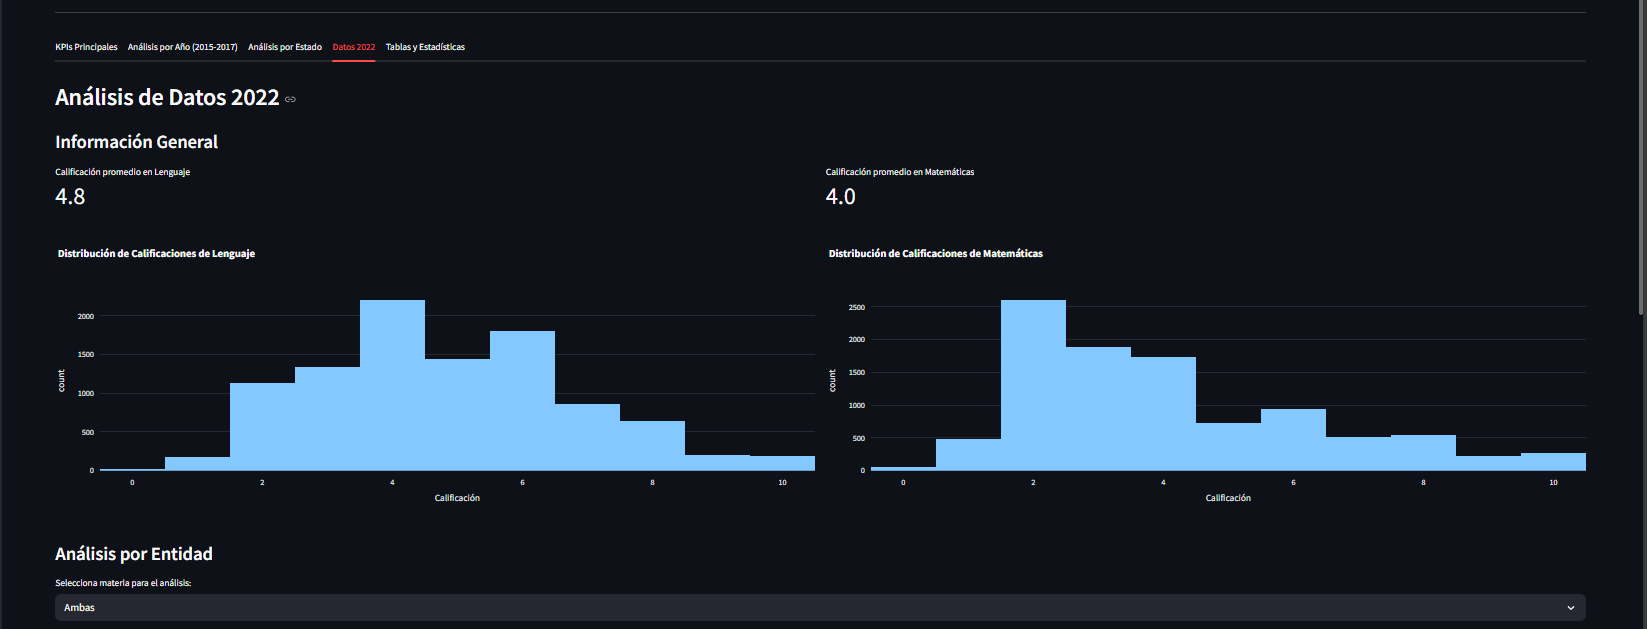
\includegraphics[width=0.8\textwidth]{../imagenes/analisis 2022.png}
    \caption{Ejemplo de histograma en el dashboard para datos 2022}
    \label{fig:histograma}
\end{figure}

\subsection{Gráficos de Correlación}
Para análisis de relaciones entre variables, se implementaron matrices de correlación:

\begin{lstlisting}[language=Python, caption=Implementación de matrices de correlación]
# Seleccionar variables numéricas para correlación
variables_seleccionadas = st.multiselect("Selecciona variables para la correlación:", 
                                        [col for col in df_año.columns if df_año[col].dtype in ['int64', 'float64']])

if variables_seleccionadas:
    # Calcular matriz de correlación
    corr_matrix = df_año[variables_seleccionadas].corr()
    
    # Visualizar como heatmap
    fig = px.imshow(
        corr_matrix,
        text_auto=True,
        aspect="auto",
        color_continuous_scale="RdBu_r",
        title=f"Matriz de correlación para variables seleccionadas ({anio_seleccionado})"
    )
    st.plotly_chart(fig, use_container_width=True)
\end{lstlisting}

Beneficios de esta visualización:
\begin{itemize}
    \item Identificación de relaciones entre variables educativas
    \item Descubrimiento de patrones no evidentes en análisis univariados
    \item Base para análisis más profundos de causalidad
\end{itemize}

\begin{figure}[h]
    \centering
    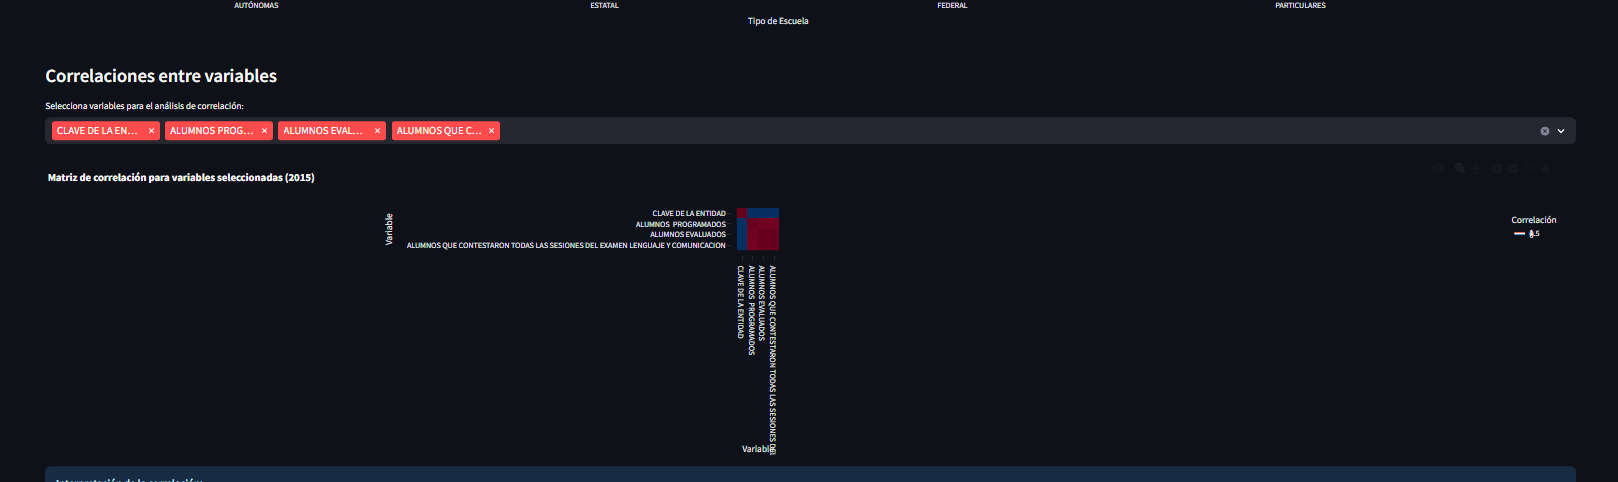
\includegraphics[width=0.8\textwidth]{../imagenes/correlaciones entre variables.png}
    \caption{Ejemplo de matriz de correlación en el dashboard}
    \label{fig:matriz_correlacion}
\end{figure}

\subsection{Tablas Interactivas}
Las tablas interactivas permiten explorar datos detallados:

\begin{lstlisting}[language=Python, caption=Implementación de tablas interactivas]
# Función para destacar filas
def highlight_row(row):
    if row["Entidad"] == entidad_seleccionada:
        return ['background-color: #FFFF00'] * len(row)
    return [''] * len(row)

# Aplicar estilo y mostrar
df_ranking_display = df_ranking.style.apply(highlight_row, axis=1)
st.dataframe(df_ranking_display[["Posición", "Entidad", "Porcentaje"]], height=400)
\end{lstlisting}

Características implementadas:
\begin{itemize}
    \item Ordenamiento dinámico por columnas
    \item Resaltado de filas relevantes
    \item Paginación para grandes conjuntos de datos
    \item Filtrado interactivo
\end{itemize}

\begin{figure}[h]
    \centering
    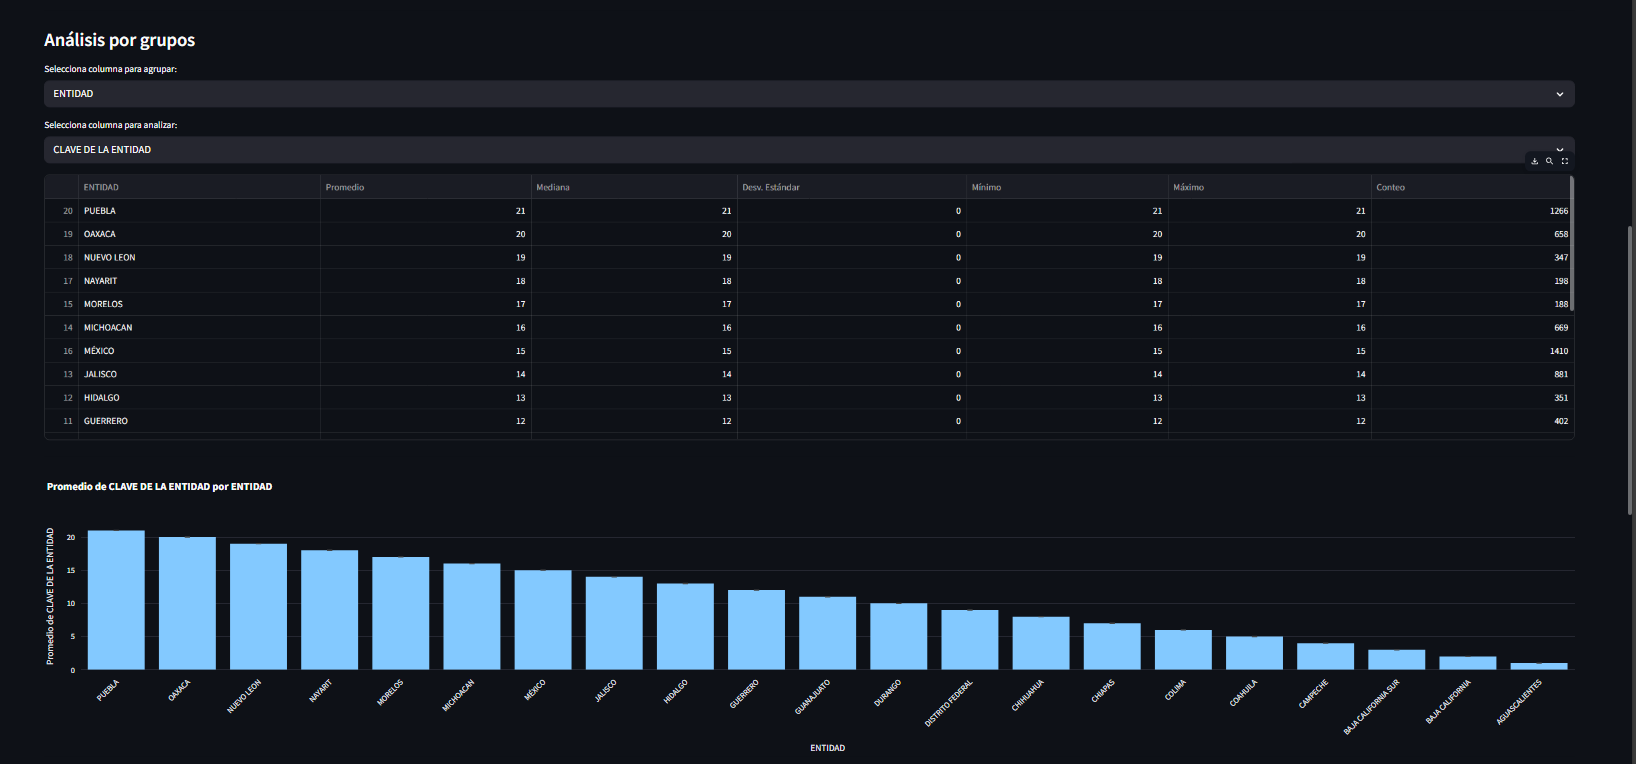
\includegraphics[width=0.8\textwidth]{../imagenes/analisis por gruoi.png}
    \caption{Ejemplo de tabla interactiva en el dashboard}
    \label{fig:tabla_interactiva}
\end{figure}

\subsection{Control de Carga de Datos}
Para optimizar el rendimiento del dashboard, especialmente con grandes volúmenes de datos, se implementó un sistema de control de carga.

\begin{figure}[h]
    \centering
    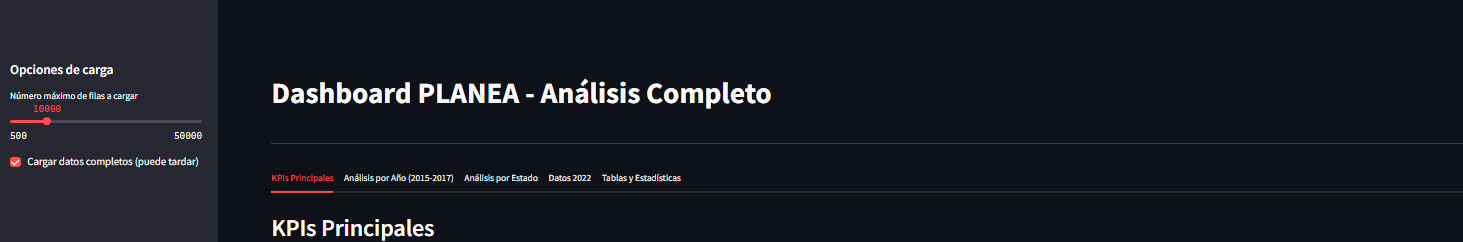
\includegraphics[width=0.8\textwidth]{../imagenes/opciones de carga.png}
    \caption{Opciones de control para la carga de datos en el dashboard}
    \label{fig:opciones_carga}
\end{figure}

\subsection{Pestaña 3: Análisis por Estado}
Dedicada al análisis geográfico:

\begin{itemize}
    \item \textbf{Evolución de la entidad}: Gráfico de línea mostrando tendencias para la entidad seleccionada.
    
    \item \textbf{Comparativa con el promedio nacional}: Contraste entre la entidad seleccionada y la media nacional.
    
    \item \textbf{Ranking nacional}: Tabla que muestra la posición relativa de cada entidad.
\end{itemize}

\begin{figure}[h]
    \centering
    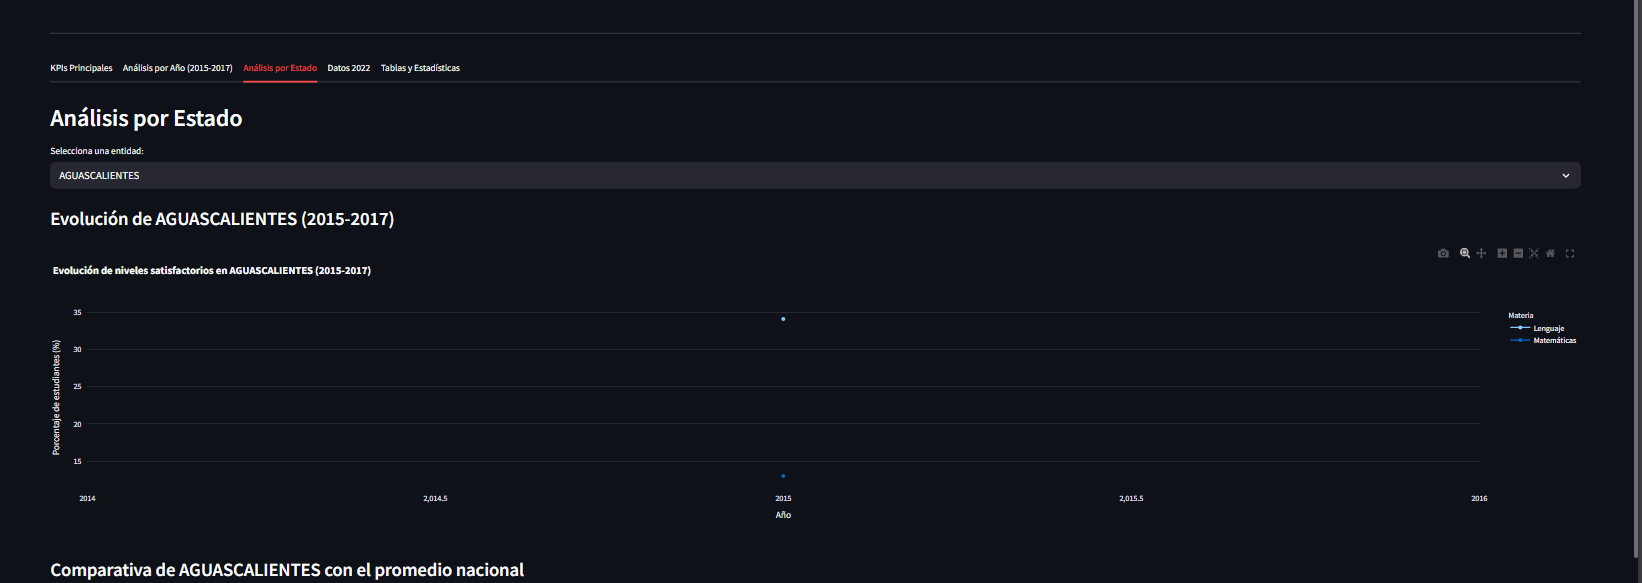
\includegraphics[width=0.8\textwidth]{../imagenes/ananlisis por estado .png}
    \caption{Análisis por estado mostrando comparativas y rankings}
    \label{fig:analisis_estado}
\end{figure}

\begin{figure}[h]
    \centering
    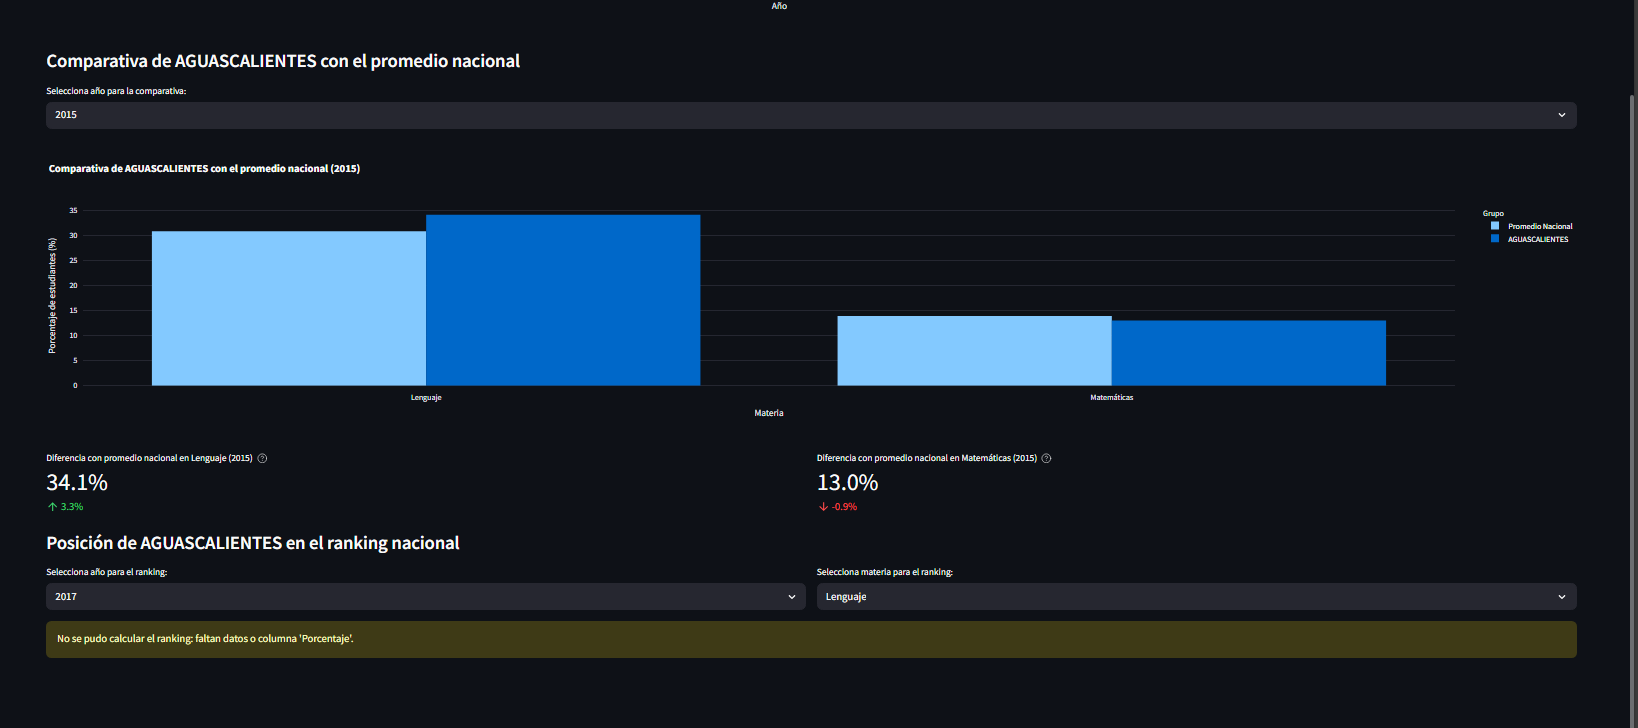
\includegraphics[width=0.8\textwidth]{../imagenes/comparativa con promedio nacioanal.png}
    \caption{Comparativa del desempeño de entidades con el promedio nacional}
    \label{fig:comparativa_nacional}
\end{figure}

\subsection{Pestaña 4: Datos 2022}
Enfocada en los datos más recientes:

\begin{itemize}
    \item \textbf{Información general}: Calificaciones promedio en Lenguaje y Matemáticas.
{{ ... }}
    \item \textbf{Análisis por entidad}: Gráficos de barras comparando entidades.
    \item \textbf{Nota comparativa}: Advertencia sobre las limitaciones de comparabilidad con años anteriores.
\end{itemize}

\begin{figure}[h]
    \centering
    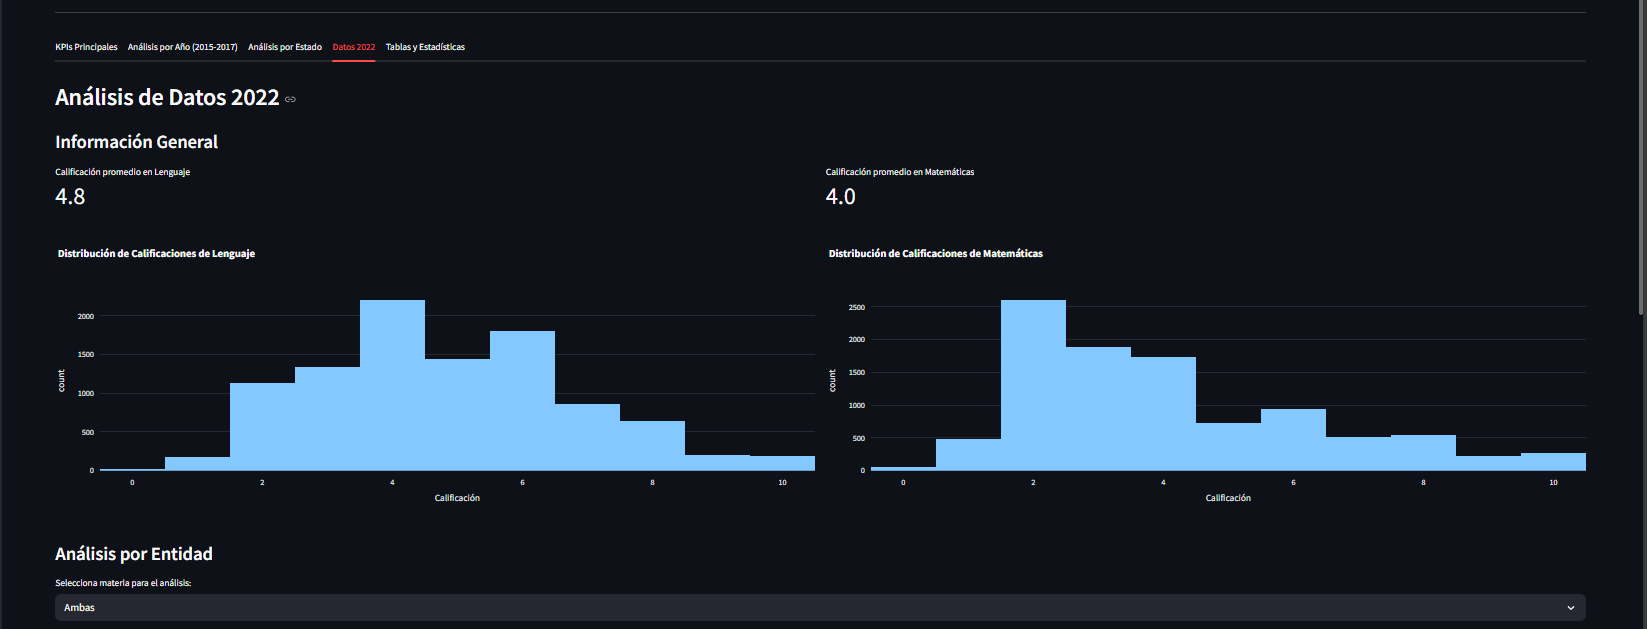
\includegraphics[width=0.8\textwidth]{../imagenes/analisis 2022.png}
    \caption{Distribución de calificaciones en Lenguaje y Matemáticas (2022)}
    \label{fig:histograma_2022}
\end{figure}

\subsection{Pestaña 5: Tablas y Estadísticas}
Proporciona acceso a datos más detallados:

\begin{itemize}
    \item \textbf{Previsualizaciones de datos}: Tablas mostrando las primeras filas de cada conjunto de datos.
    \item \textbf{Estadísticas descriptivas}: Resúmenes estadísticos calculados con \texttt{df.describe()}.
    \item \textbf{Análisis por grupos}: Estadísticas agrupadas por variables seleccionadas.
    \item \textbf{Filtrado personalizado}: Herramientas para crear subconjuntos específicos.
\end{itemize}

\begin{figure}[h]
    \centering
    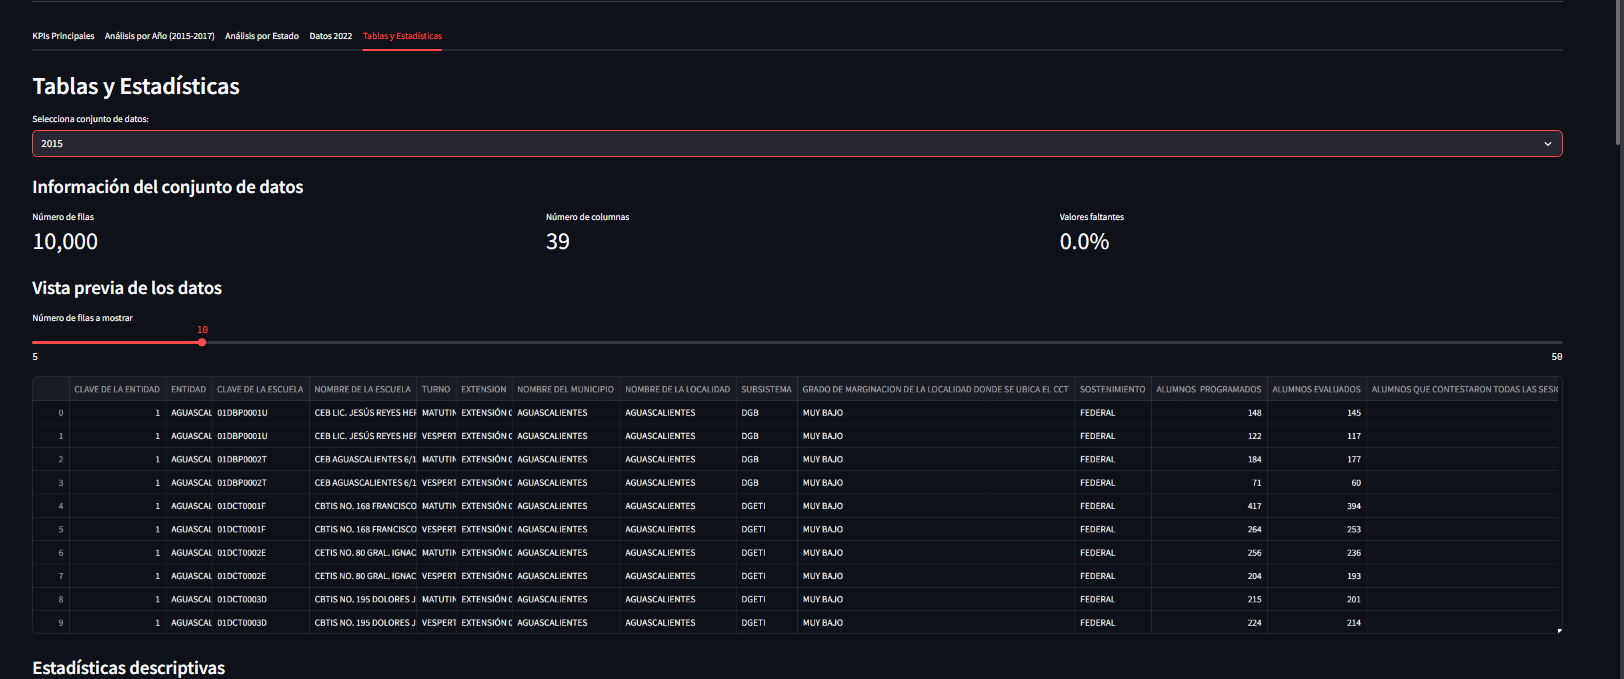
\includegraphics[width=0.8\textwidth]{../imagenes/tabla y estadisticas.png}
    \caption{Tablas y estadísticas descriptivas de los datos}
    \label{fig:tablas_estadisticas}
\end{figure}

\begin{figure}[h]
    \centering
    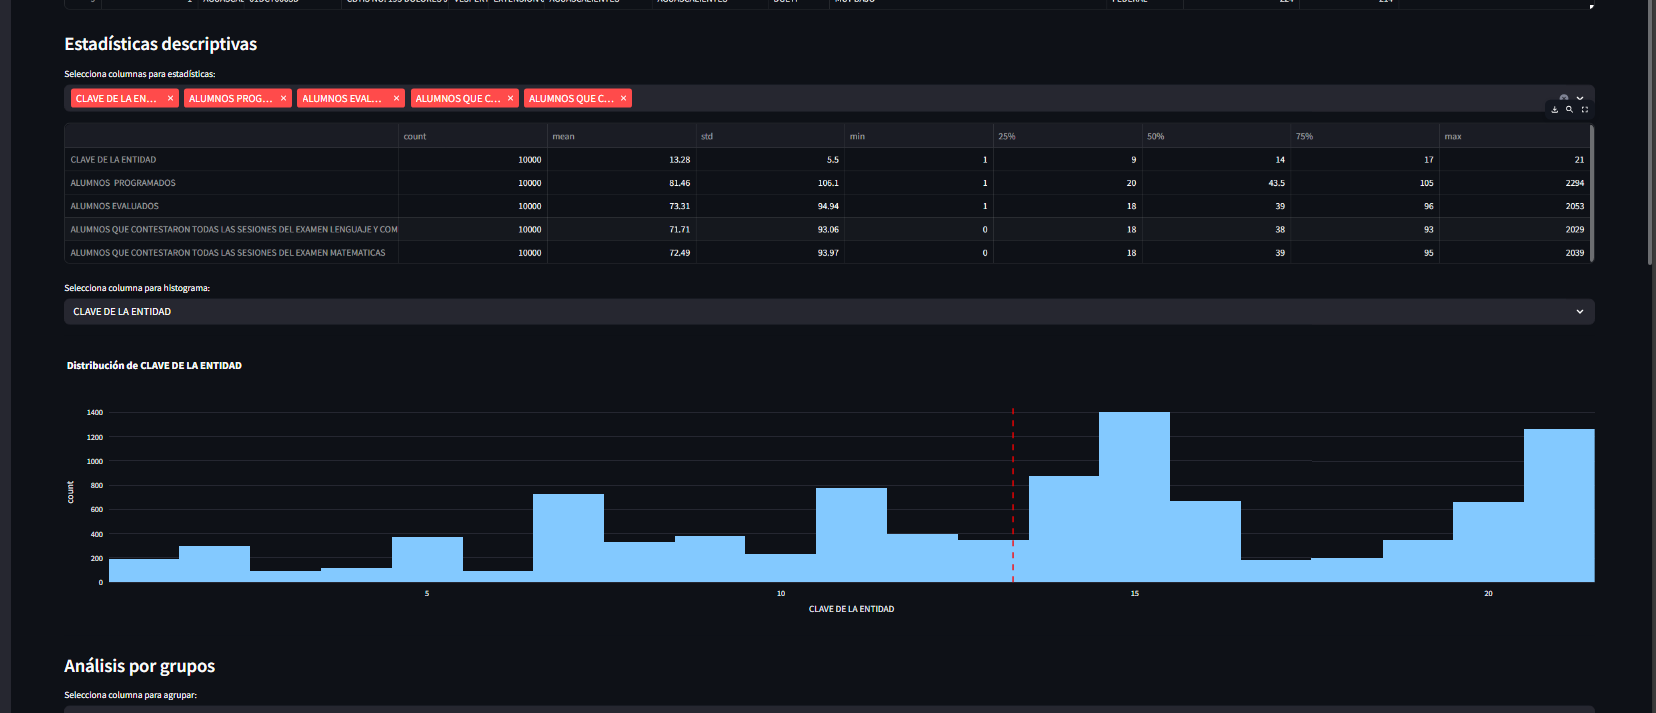
\includegraphics[width=0.8\textwidth]{../imagenes/estadisticas descripticas.png}
    \caption{Resúmenes estadísticos detallados de las variables numéricas}
    \label{fig:estadisticas_descriptivas}
\end{figure}

\section{Interactividad y Filtros}

\begin{figure}[h]
    \centering
    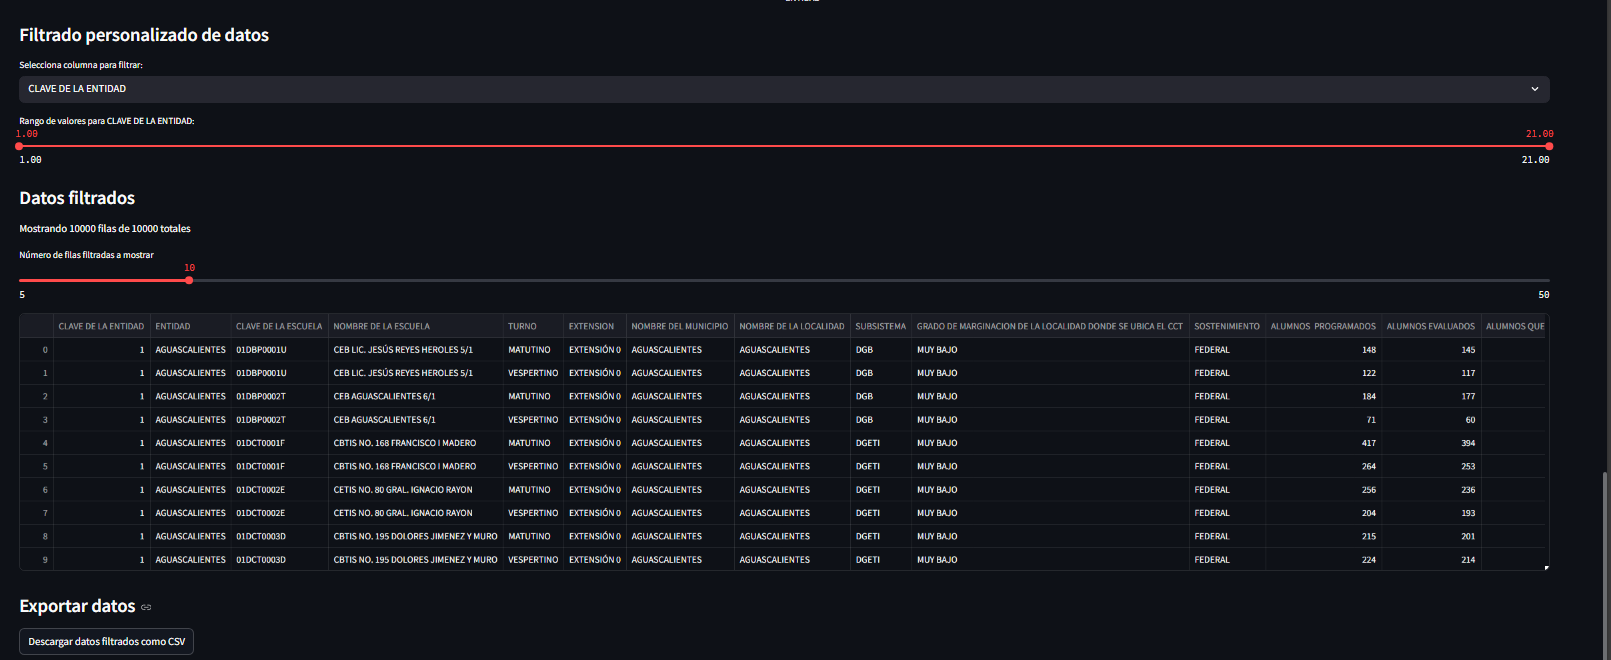
\includegraphics[width=0.8\textwidth]{../imagenes/filtrado de datos.png}
    \caption{Opciones de filtrado interactivo en el dashboard}
    \label{fig:filtrado_datos}
\end{figure}

\subsection{Selectores Implementados}
El dashboard incorpora diversos elementos interactivos:

\begin{lstlisting}[language=Python, caption=Implementación de selectores]
# Selector de año
anio_seleccionado = st.selectbox("Selecciona un año para analizar:", [2015, 2016, 2017])

# Selector de tipo de escuela
tipo_escuela = st.selectbox("Selecciona un tipo de escuela:", ["AUTÓNOMAS", "ESTATAL", "FEDERAL", "PARTICULARES"])

# Selector de entidad
entidad_seleccionada = st.selectbox("Selecciona una entidad:", entidades)

# Selector múltiple para variables
variables = st.multiselect("Selecciona variables para el análisis:", columnas_numericas)
\end{lstlisting}

\subsection{Filtros Dinámicos}
Los filtros se implementan de forma dinámica:

\begin{lstlisting}[language=Python, caption=Implementación de filtros dinámicos]
# Filtro por entidad
df_filtrado = df[df[entidad_col] == entidad_seleccionada]

# Filtro por año
df_filtrado = df[df["AÑO"] == anio_seleccionado]

# Filtro por tipo de escuela
df_filtrado = df[df["TIPO DE ESCUELA"] == tipo_escuela]

# Filtro personalizado con slider
valor_minimo = st.slider("Filtrar por valor mínimo:", 
                         min_value=float(df[columna].min()), 
                         max_value=float(df[columna].max()))
df_filtrado = df[df[columna] >= valor_minimo]
\end{lstlisting}

\subsection{Elementos Interactivos en Visualizaciones}
Las visualizaciones incluyen elementos interactivos avanzados:

\begin{itemize}
    \item \textbf{Tooltips}: Información detallada al pasar el cursor sobre elementos gráficos.
    \item \textbf{Zoom}: Capacidad para ampliar áreas específicas de los gráficos.
    \item \textbf{Selección}: Posibilidad de seleccionar elementos específicos para análisis detallado.
    \item \textbf{Leyendas interactivas}: Clic en leyendas para mostrar/ocultar series.
    \item \textbf{Botones de descarga}: Opción para guardar gráficos como imágenes.
\end{itemize}

\section{Personalización Visual}

\subsection{Paleta de Colores}
Se implementó una paleta de colores consistente:

\begin{itemize}
    \item \textbf{Colores primarios}: Azul claro y azul oscuro para las dos materias principales.
    \item \textbf{Colores de contraste}: Rojo y verde para indicadores de cambio.
    \item \textbf{Colores neutros}: Grises para elementos secundarios.
    \item \textbf{Destacados}: Amarillo para resaltar elementos seleccionados.
\end{itemize}

\subsection{Temas y Estilos}
El dashboard utiliza un tema oscuro para mejorar la legibilidad y reducir la fatiga visual:

\begin{lstlisting}[language=Python, caption=Configuración de tema]
# Tema oscuro predeterminado en Streamlit
# Personalización adicional de elementos
st.markdown("""
<style>
    .metric-label { font-size: 0.8rem !important; }
    .metric-value { font-weight: bold !important; }
    .warning { background-color: rgba(255, 190, 0, 0.2); padding: 10px; border-radius: 5px; }
</style>
""", unsafe_allow_html=True)
\end{lstlisting}

\section{Accesibilidad y Usabilidad}

\subsection{Consideraciones de Accesibilidad}
Se implementaron diversas características para mejorar la accesibilidad:

\begin{itemize}
    \item \textbf{Contraste adecuado}: Asegurar legibilidad para personas con baja visión.
    \item \textbf{Textos alternativos}: Descripciones para elementos visuales.
    \item \textbf{Paleta amigable para daltonismo}: Selección de colores distinguibles por personas con daltonismo.
    \item \textbf{Estructura jerárquica}: Organización lógica para lectores de pantalla.
\end{itemize}

\subsection{Mejoras de Usabilidad}
Para optimizar la experiencia de usuario:

\begin{itemize}
    \item \textbf{Mensajes de ayuda}: Tooltips y explicaciones sobre funcionalidades.
    \item \textbf{Retroalimentación visual}: Indicadores claros de estados y acciones.
    \item \textbf{Consistencia}: Patrones de interacción similares en todo el dashboard.
    \item \textbf{Mensajes de error informativos}: Comunicación clara cuando algo no funciona.
\end{itemize}

\section{Desafíos y Soluciones}

\subsection{Visualización de Datos Incompletos}
Para manejar datos faltantes en las visualizaciones:

\begin{itemize}
    \item \textbf{Advertencias visuales}: Mensajes claros cuando faltan datos.
    \item \textbf{Visualizaciones adaptativas}: Gráficos que se ajustan a datos parciales.
    \item \textbf{Indicadores de completitud}: Información sobre qué porcentaje de datos está disponible.
\end{itemize}

\subsection{Comparabilidad Visual entre Períodos}
Para abordar los desafíos de visualización entre datos 2015-2017 y 2022:

\begin{itemize}
    \item \textbf{Etiquetas diferenciadoras}: Distinción clara entre porcentajes y calificaciones promedio.
    \item \textbf{Escalas separadas}: Uso de ejes diferentes cuando es necesario.
    \item \textbf{Notas contextuales}: Información clara sobre cambios metodológicos.
    \item \textbf{Visualizaciones paralelas}: Presentación lado a lado en lugar de superpuesta cuando es apropiado.
\end{itemize}

\section{Evaluación de Efectividad}

\subsection{Criterios de Evaluación}
Las visualizaciones fueron evaluadas según los siguientes criterios:

\begin{itemize}
    \item \textbf{Precisión}: Representación fiel de los datos subyacentes.
    \item \textbf{Claridad}: Facilidad de comprensión para usuarios diversos.
    \item \textbf{Eficiencia}: Cantidad de información transmitida por unidad de espacio.
    \item \textbf{Contextualización}: Presencia de elementos que facilitan la interpretación.
    \item \textbf{Estética}: Atractivo visual sin comprometer la funcionalidad.
\end{itemize}

\subsection{Mejoras Iterativas}
El diseño visual evolucionó a través de un proceso iterativo:

\begin{itemize}
    \item \textbf{Revisión de literatura}: Incorporación de mejores prácticas de visualización de datos educativos.
    \item \textbf{Pruebas con usuarios}: Ajustes basados en retroalimentación de usuarios potenciales.
    \item \textbf{Análisis de interacción}: Optimización basada en patrones de uso observados.
    \item \textbf{Refinamiento técnico}: Mejoras en rendimiento y precisión de visualizaciones.
\end{itemize}

En conclusión, las visualizaciones implementadas en el dashboard PLANEA representan un balance entre rigor analítico, claridad comunicativa y usabilidad, permitiendo a usuarios con diferentes niveles de experiencia extraer información valiosa sobre el desempeño educativo en México a través de los años evaluados.

\chapter{Resultados y Análisis}

\section{Panorama General del Desempeño Educativo}
Los resultados obtenidos a través del dashboard PLANEA proporcionan un panorama integral del desempeño educativo en México durante los períodos 2015-2017 y 2022, revelando patrones, tendencias y desafíos significativos en el sistema educativo nacional.

\subsection{Desempeño Nacional}
A nivel nacional, los datos analizados muestran las siguientes tendencias generales:

\begin{itemize}
    \item \textbf{Niveles satisfactorios (2015-2017)}: El porcentaje de estudiantes que alcanzaron niveles satisfactorios (III y IV) se mantuvo consistentemente bajo, oscilando entre 15\% y 25\% dependiendo del año y la materia.
    
    \item \textbf{Diferencia entre materias}: Se observa una brecha persistente entre Lenguaje y Matemáticas, con esta última mostrando resultados sistemáticamente inferiores.
    
    \item \textbf{Evolución temporal}: Entre 2015 y 2017 se observaron mejoras modestas pero consistentes en ambas materias, con un incremento promedio de 1-2 puntos porcentuales por año.
    
    \item \textbf{Calificaciones 2022}: Las calificaciones promedio nacionales para 2022 reflejan la persistencia de desafíos educativos, aunque la diferente metodología limita comparaciones directas con el período anterior.
\end{itemize}

\begin{figure}[h]
    \centering
    % Incluir la imagen del gráfico nacional cuando esté disponible
    % \includegraphics[width=0.8\textwidth]{../imagenes/tendencia_nacional.png}
    \caption{Evolución del porcentaje de estudiantes en niveles satisfactorios a nivel nacional (2015-2017)}
    \label{fig:tendencia_nacional}
\end{figure}

\section{Análisis por Tipo de Escuela}
El análisis por tipo de escuela revela disparidades significativas en el sistema educativo mexicano.

\subsection{Desempeño Comparativo}
Los resultados muestran un patrón consistente en la jerarquía de desempeño entre los diferentes tipos de escuela:

\begin{itemize}
    \item \textbf{Escuelas particulares}: Consistentemente obtienen los mejores resultados, con porcentajes de niveles satisfactorios que duplican o triplican el promedio nacional.
    
    \item \textbf{Escuelas autónomas}: Ocupan el segundo lugar en desempeño, con resultados moderadamente superiores al promedio nacional.
    
    \item \textbf{Escuelas federales}: Presentan resultados cercanos al promedio nacional, con variaciones según el año y la materia.
    
    \item \textbf{Escuelas estatales}: Tienden a mostrar los resultados más bajos, especialmente en Matemáticas.
\end{itemize}

\subsection{Brechas de Desigualdad}
El análisis cuantifica las brechas educativas:

\begin{itemize}
    \item La diferencia entre escuelas particulares y estatales en porcentaje de niveles satisfactorios alcanza hasta 30 puntos porcentuales en algunos casos.
    
    \item Esta brecha se ha mantenido relativamente estable durante el período analizado, sin signos claros de reducción.
    
    \item En 2022, las calificaciones promedio muestran patrones similares de desigualdad, sugiriendo la persistencia de estos desafíos estructurales.
\end{itemize}

\begin{figure}[h]
    \centering
    % \includegraphics[width=0.8\textwidth]{../imagenes/comparativa_tipos_escuela.png}
    \caption{Comparativa de desempeño por tipo de escuela (2017)}
    \label{fig:comparativa_tipos}
\end{figure}

\section{Análisis Geográfico}
El análisis por entidad federativa revela importantes disparidades regionales en el desempeño educativo.

\subsection{Distribución Geográfica del Desempeño}
Los resultados muestran patrones geográficos consistentes:

\begin{itemize}
    \item \textbf{Entidades de alto desempeño}: Ciudad de México, Aguascalientes, Querétaro y Jalisco tienden a posicionarse consistentemente en los primeros lugares.
    
    \item \textbf{Entidades de bajo desempeño}: Chiapas, Guerrero, Tabasco y Michoacán frecuentemente aparecen en las últimas posiciones.
    
    \item \textbf{Correlación con desarrollo socioeconómico}: Se observa una correlación positiva entre el desempeño educativo y diversos indicadores de desarrollo económico y social.
\end{itemize}

\subsection{Casos de Éxito y Rezago}
El análisis detallado identifica casos particulares de interés:

\begin{itemize}
    \item \textbf{Casos de mejora destacada}: Entidades como Sonora y Sinaloa mostraron mejoras sostenidas superiores al promedio nacional durante 2015-2017.
    
    \item \textbf{Casos de estancamiento}: Algunas entidades como Oaxaca presentaron poca o nula mejora durante el período estudiado.
    
    \item \textbf{Brecha máxima}: La diferencia entre la entidad mejor y peor posicionada llega a superar los 20 puntos porcentuales en niveles satisfactorios.
\end{itemize}

\begin{figure}[h]
    \centering
    % \includegraphics[width=0.8\textwidth]{../imagenes/ranking_entidades.png}
    \caption{Ranking de entidades por porcentaje en niveles satisfactorios (2017)}
    \label{fig:ranking_entidades}
\end{figure}

\section{Análisis de Correlaciones}
El análisis de correlaciones revela relaciones significativas entre diferentes variables educativas.

\subsection{Correlaciones entre Materias}
Las correlaciones entre desempeño en diferentes materias muestran:

\begin{itemize}
    \item Una correlación positiva fuerte (r > 0.8) entre el desempeño en Lenguaje y Matemáticas, tanto en 2015-2017 como en 2022.
    
    \item Esta correlación sugiere que los factores que influyen en el aprendizaje tienden a afectar de manera similar a ambas materias.
    
    \item Sin embargo, la intensidad de esta correlación varía según el tipo de escuela, siendo más fuerte en escuelas particulares y más débil en escuelas estatales.
\end{itemize}

\subsection{Correlaciones con Variables Socioeconómicas}
El análisis de correlaciones con factores contextuales revela:

\begin{itemize}
    \item Correlación positiva moderada a fuerte entre el nivel socioeconómico de la escuela y el porcentaje de niveles satisfactorios.
    
    \item Correlación negativa entre indicadores de marginación y el desempeño educativo.
    
    \item Estas correlaciones apuntan a la persistencia de desafíos de equidad en el sistema educativo mexicano.
\end{itemize}

\begin{figure}[h]
    \centering
    % \includegraphics[width=0.8\textwidth]{../imagenes/matriz_correlacion.png}
    \caption{Matriz de correlación entre variables educativas clave (2017)}
    \label{fig:matriz_correlacion}
\end{figure}

\section{Análisis de los Datos 2022}

\subsection{Distribución de Calificaciones}
El análisis de los datos de 2022 muestra patrones distintivos:

\begin{itemize}
    \item Las distribuciones de calificaciones en ambas materias presentan una forma aproximadamente normal, con ligera asimetría negativa.
    
    \item La dispersión (desviación estándar) es mayor en Matemáticas que en Lenguaje, sugiriendo mayores disparidades en esta materia.
    
    \item Se observan diferencias significativas en las medias por tipo de escuela, replicando patrones similares a los observados en 2015-2017.
\end{itemize}

\subsection{Comparativa con Períodos Anteriores}
Aunque la comparación directa es limitada, se pueden extraer algunas conclusiones:

\begin{itemize}
    \item La jerarquía de desempeño entre tipos de escuela se mantiene consistente con el período 2015-2017.
    
    \item La distribución geográfica del desempeño muestra patrones similares, con las mismas entidades tendiendo a aparecer en extremos superiores e inferiores.
    
    \item Esto sugiere que, a pesar de los cambios metodológicos en la evaluación, las desigualdades estructurales en el sistema educativo persisten.
\end{itemize}

\begin{figure}[h]
    \centering
    % \includegraphics[width=0.8\textwidth]{../imagenes/histograma_2022.png}
    \caption{Distribución de calificaciones en Lenguaje y Matemáticas (2022)}
    \label{fig:histograma_2022}
\end{figure}

\section{Tendencias y Patrones Longitudinales}

\subsection{Evolución del Desempeño 2015-2017}
El análisis longitudinal para el período 2015-2017 revela:

\begin{itemize}
    \item Un incremento moderado pero sostenido en el porcentaje de estudiantes en niveles satisfactorios.
    
    \item La tasa de mejora fue ligeramente mayor en Matemáticas que en Lenguaje, aunque partiendo de niveles iniciales más bajos.
    
    \item Las brechas entre tipos de escuela y entre entidades se mantuvieron relativamente estables durante este período.
\end{itemize}

\subsection{Patrones Consistentes}
A lo largo de todos los períodos analizados, se observan patrones consistentes:

\begin{itemize}
    \item La persistencia de desigualdades educativas correlacionadas con factores socioeconómicos y geográficos.
    
    \item Desafíos particulares en el área de Matemáticas, con resultados sistemáticamente inferiores a los de Lenguaje.
    
    \item Mayor variabilidad en los resultados de escuelas estatales y federales comparadas con particulares, sugiriendo mayor heterogeneidad en el sector público.
\end{itemize}

\section{Implicaciones para Políticas Educativas}

\subsection{Áreas Prioritarias Identificadas}
El análisis permite identificar áreas que requieren atención prioritaria:

\begin{itemize}
    \item \textbf{Fortalecimiento de Matemáticas}: Los resultados consistentemente más bajos en esta materia señalan la necesidad de estrategias específicas.
    
    \item \textbf{Reducción de brechas}: Las persistentes disparidades entre tipos de escuela y regiones demandan políticas compensatorias.
    
    \item \textbf{Atención a entidades rezagadas}: Las entidades con desempeño consistentemente bajo requieren intervenciones focalizadas.
    
    \item \textbf{Aprovechamiento de casos exitosos}: Estudiar y potencialmente replicar estrategias de entidades que han mostrado mejoras significativas.
\end{itemize}

\subsection{Evaluación de Políticas Existentes}
Los datos permiten una evaluación preliminar de políticas educativas:

\begin{itemize}
    \item Las mejoras moderadas en 2015-2017 sugieren efectos positivos pero limitados de las políticas implementadas en ese período.
    
    \item La persistencia de brechas apunta a la insuficiencia de los mecanismos de compensación y equidad existentes.
    
    \item Los patrones observados en 2022 indican que los desafíos estructurales continúan presentes a pesar de cambios en políticas educativas.
\end{itemize}

\section{Hallazgos Clave}

Los hallazgos más significativos derivados del análisis pueden resumirse en:

\begin{enumerate}
    \item \textbf{Bajo nivel general}: El porcentaje de estudiantes que alcanzan niveles satisfactorios es consistentemente bajo a nivel nacional, indicando desafíos fundamentales en la calidad educativa.
    
    \item \textbf{Desigualdades persistentes}: Existen brechas significativas y persistentes entre tipos de escuela y regiones geográficas, reflejando y potencialmente reforzando desigualdades socioeconómicas.
    
    \item \textbf{Mejoras graduales}: Entre 2015 y 2017 se observaron mejoras modestas pero consistentes, sugiriendo un progreso lento pero positivo.
    
    \item \textbf{Desafío en Matemáticas}: El desempeño en Matemáticas es sistemáticamente inferior al de Lenguaje, señalando desafíos particulares en esta área.
    
    \item \textbf{Correlación socioeconómica}: Existe una correlación significativa entre factores socioeconómicos y desempeño educativo, subrayando la influencia del contexto en los resultados.
    
    \item \textbf{Continuidad de patrones}: Los datos de 2022, a pesar de diferencias metodológicas, muestran la persistencia de patrones similares de desigualdad y desafíos.
\end{enumerate}

Estos hallazgos proporcionan una base empírica sólida para la formulación de políticas educativas más efectivas y focalizadas, orientadas a mejorar la calidad educativa y reducir las brechas de desigualdad en el sistema educativo mexicano.

\chapter{Limitaciones y Consideraciones}

\section{Limitaciones de los Datos}
Los datos utilizados en el dashboard PLANEA presentan diversas limitaciones que deben tenerse en cuenta al interpretar los resultados y conclusiones derivadas del análisis.

\subsection{Cambios Metodológicos entre Períodos}
Una de las limitaciones más significativas es la diferencia metodológica entre los períodos 2015-2017 y 2022:

\begin{itemize}
    \item \textbf{Diferencias en estructura}: Los datos de 2015-2017 presentan información sobre distribución por niveles de logro, mientras que los de 2022 solo proporcionan calificaciones directas.
    
    \item \textbf{Cambios en escalas}: La escala utilizada para 2022 no es directamente comparable con los porcentajes de niveles de 2015-2017.
    
    \item \textbf{Impacto en comparabilidad}: Estas diferencias limitan severamente la posibilidad de realizar comparaciones directas de desempeño entre ambos períodos.
\end{itemize}

\subsection{Datos Ausentes}
El análisis está afectado por la presencia de datos ausentes en diversos contextos:

\begin{itemize}
    \item \textbf{Ausencia de años intermedios}: No se dispone de datos para 2018-2021, creando un vacío temporal significativo en el análisis longitudinal.
    
    \item \textbf{Datos faltantes por entidad}: Algunas entidades presentan datos incompletos para ciertos años o tipos de escuela.
    
    \item \textbf{Vacíos en variables contextuales}: Información limitada sobre factores socioeconómicos, recursos escolares y características docentes que podrían enriquecer el análisis.
\end{itemize}

\subsection{Representatividad}
Es importante considerar las limitaciones en la representatividad de los datos:

\begin{itemize}
    \item \textbf{Cobertura incompleta}: Las evaluaciones PLANEA no cubren la totalidad de la población estudiantil, particularmente en zonas remotas o marginadas.
    
    \item \textbf{Exclusión de ciertos sectores}: Estudiantes con discapacidades severas, en situación de calle o que han abandonado el sistema educativo no están representados.
    
    \item \textbf{Sesgo de participación}: Posible subrepresentación de escuelas con menores recursos o capacidades organizativas para implementar adecuadamente las evaluaciones.
\end{itemize}

\section{Limitaciones Técnicas del Dashboard}

\subsection{Restricciones de Procesamiento}
El dashboard enfrenta algunas limitaciones técnicas que afectan su funcionamiento:

\begin{itemize}
    \item \textbf{Volumen de datos}: El procesamiento de conjuntos completos de datos puede resultar lento en equipos con recursos limitados.
    
    \item \textbf{Implementación de caché}: Aunque se implementó caché para mejorar el rendimiento, ciertas operaciones siguen requiriendo recálculo frecuente.
    
    \item \textbf{Limitaciones de memoria}: El manejo de grandes volúmenes de datos está restringido por la memoria disponible, requiriendo controles de carga como el limitador de filas.
\end{itemize}

\subsection{Limitaciones de Visualización}
Las visualizaciones implementadas presentan ciertas restricciones:

\begin{itemize}
    \item \textbf{Densidad de información}: Algunas visualizaciones complejas pueden resultar difíciles de interpretar para usuarios no especializados.
    
    \item \textbf{Representación geográfica}: Ausencia de visualizaciones geoespaciales detalladas que podrían enriquecer el análisis territorial.
    
    \item \textbf{Visualizaciones avanzadas}: Carencia de técnicas de visualización más sofisticadas como análisis de redes, mapas de calor multidimensionales o visualizaciones interactivas complejas.
\end{itemize}

\subsection{Accesibilidad}
A pesar de los esfuerzos por mejorar la accesibilidad, persisten algunas limitaciones:

\begin{itemize}
    \item \textbf{Dependencia visual}: El dashboard depende fundamentalmente de representaciones visuales, lo que puede limitar su utilidad para personas con discapacidad visual.
    
    \item \textbf{Complejidad cognitiva}: Algunos análisis requieren conocimientos estadísticos o educativos específicos para su correcta interpretación.
    
    \item \textbf{Barreras tecnológicas}: Requiere acceso a dispositivos con capacidades técnicas mínimas y conexión a internet.
\end{itemize}

\section{Limitaciones Analíticas}

\subsection{Causalidad vs. Correlación}
Una limitación importante del análisis es la dificultad para establecer relaciones causales:

\begin{itemize}
    \item \textbf{Correlaciones observadas}: El dashboard identifica numerosas correlaciones entre variables, pero no permite determinar causalidad.
    
    \item \textbf{Variables omitidas}: Posible existencia de factores no medidos que podrían explicar las relaciones observadas.
    
    \item \textbf{Direccionalidad}: Dificultad para determinar la dirección de influencia en las relaciones identificadas.
\end{itemize}

\subsection{Granularidad del Análisis}
El nivel de detalle del análisis está limitado por la estructura de los datos disponibles:

\begin{itemize}
    \item \textbf{Nivel escolar}: Los datos no permiten análisis a nivel de aula o estudiante individual, que podrían revelar patrones más específicos.
    
    \item \textbf{Factores pedagógicos}: Ausencia de información detallada sobre prácticas pedagógicas, metodologías didácticas o experiencia docente.
    
    \item \textbf{Contexto local}: Información limitada sobre características específicas del contexto local que pueden influir en los resultados.
\end{itemize}

\subsection{Complejidad del Fenómeno Educativo}
El análisis cuantitativo captura solo parcialmente la complejidad del fenómeno educativo:

\begin{itemize}
    \item \textbf{Dimensiones no académicas}: Aspectos socioemocionales, creatividad, pensamiento crítico y otras dimensiones importantes del aprendizaje no son capturados.
    
    \item \textbf{Contexto histórico-cultural}: Limitada consideración de factores históricos, culturales y lingüísticos que influyen en los procesos educativos.
    
    \item \textbf{Validez de las pruebas}: Cuestionamientos sobre la capacidad de las pruebas estandarizadas para medir adecuadamente el aprendizaje significativo.
\end{itemize}

\section{Consideraciones Éticas}

\subsection{Interpretación Responsable}
Es fundamental promover una interpretación responsable de los resultados:

\begin{itemize}
    \item \textbf{Riesgo de simplificación}: Los datos cuantitativos pueden llevar a simplificaciones excesivas de fenómenos educativos complejos.
    
    \item \textbf{Estigmatización}: Existe el riesgo de estigmatizar a entidades, escuelas o grupos con menor desempeño sin considerar su contexto particular.
    
    \item \textbf{Narrativas deterministas}: Es importante evitar narrativas que sugieran un determinismo social o geográfico en el desempeño educativo.
\end{itemize}

\subsection{Uso de Datos}
El uso responsable de los datos implica considerar:

\begin{itemize}
    \item \textbf{Privacidad}: Aunque los datos son agregados, es importante mantener la confidencialidad y evitar identificaciones indirectas.
    
    \item \textbf{Consentimiento informado}: Reflexionar sobre si los participantes en las evaluaciones fueron adecuadamente informados sobre los posibles usos de sus datos.
    
    \item \textbf{Equidad en el acceso}: Considerar si el acceso a estos análisis está equitativamente distribuido entre diferentes actores educativos.
\end{itemize}

\subsection{Impacto de las Evaluaciones}
Es necesario considerar el impacto de las evaluaciones estandarizadas:

\begin{itemize}
    \item \textbf{Presión sobre actores educativos}: Las evaluaciones pueden generar presiones indebidas sobre docentes y estudiantes.
    
    \item \textbf{"Enseñar para la prueba"}: Riesgo de que el currículum se estreche para enfocarse en contenidos evaluados.
    
    \item \textbf{Jerarquización}: Las comparaciones pueden reforzar jerarquías existentes entre instituciones educativas.
\end{itemize}

\section{Trabajo Futuro}

\subsection{Mejoras en Datos}
Para superar las limitaciones actuales, se podrían implementar las siguientes mejoras:

\begin{itemize}
    \item \textbf{Integración de nuevas fuentes}: Incorporar datos de otras evaluaciones o registros administrativos para enriquecer el análisis.
    
    \item \textbf{Desarrollo de equivalencias}: Investigar y desarrollar métodos estadísticos para establecer equivalencias aproximadas entre las diferentes escalas utilizadas.
    
    \item \textbf{Variables contextuales}: Integrar datos socioeconómicos, de infraestructura escolar y características docentes para contextualizar mejor los resultados.
\end{itemize}

\subsection{Mejoras Técnicas}
El dashboard podría beneficiarse de diversas mejoras técnicas:

\begin{itemize}
    \item \textbf{Optimización de rendimiento}: Implementar estrategias más avanzadas de caché y procesamiento paralelo.
    
    \item \textbf{Visualizaciones geoespaciales}: Incorporar mapas interactivos que permitan análisis territoriales más detallados.
    
    \item \textbf{Técnicas de aprendizaje automático}: Explorar el uso de algoritmos predictivos para identificar patrones complejos o factores de riesgo.
    
    \item \textbf{Exportación de reportes}: Desarrollar funcionalidades para generar reportes personalizados exportables.
\end{itemize}

\subsection{Ampliación del Análisis}
El análisis podría expandirse en varias direcciones:

\begin{itemize}
    \item \textbf{Análisis longitudinal de cohortes}: Seguimiento de cohortes específicas a lo largo del tiempo cuando los datos lo permitan.
    
    \item \textbf{Análisis multifactorial}: Exploración de interacciones complejas entre múltiples factores educativos y contextuales.
    
    \item \textbf{Estudios de casos atípicos}: Investigación detallada de casos que muestran resultados significativamente diferentes a lo esperado según su contexto.
    
    \item \textbf{Integración con investigación cualitativa}: Complementar el análisis cuantitativo con hallazgos de investigaciones cualitativas sobre prácticas educativas efectivas.
\end{itemize}

\section{Recomendaciones para Usuarios}

\subsection{Interpretación Contextualizada}
Se recomienda a los usuarios del dashboard:

\begin{itemize}
    \item \textbf{Considerar el contexto}: Interpretar los resultados a la luz de las características socioeconómicas, históricas y culturales específicas.
    
    \item \textbf{Atender a las advertencias}: Prestar atención a las notas y advertencias sobre limitaciones de comparabilidad y representatividad.
    
    \item \textbf{Combinar fuentes}: Complementar la información del dashboard con otras fuentes de datos educativos.
\end{itemize}

\subsection{Uso para Mejora Educativa}
Para un uso orientado a la mejora educativa:

\begin{itemize}
    \item \textbf{Enfoque en tendencias}: Priorizar el análisis de tendencias y patrones por encima de comparaciones puntuales.
    
    \item \textbf{Identificación de fortalezas}: Utilizar los datos para identificar fortalezas y prácticas efectivas, no solo áreas de mejora.
    
    \item \textbf{Base para indagación}: Considerar los hallazgos como punto de partida para investigaciones más profundas, no como conclusiones definitivas.
    
    \item \textbf{Participación de actores}: Involucrar a diversos actores educativos en la interpretación y uso de los datos para la toma de decisiones.
\end{itemize}

En conclusión, si bien el dashboard PLANEA proporciona una herramienta valiosa para el análisis del desempeño educativo en México, es fundamental reconocer sus limitaciones y utilizarlo de manera crítica y contextualizada, como un complemento —no un sustituto— del juicio profesional y la comprensión profunda de las realidades educativas locales.

\chapter{Conclusiones y Recomendaciones}

\section{Conclusiones Generales}
El desarrollo e implementación del dashboard PLANEA ha permitido obtener una visión integral y detallada del desempeño educativo en México durante los períodos 2015-2017 y 2022, generando conocimientos significativos sobre los logros, desafíos y tendencias en el sistema educativo nacional.

\subsection{Sobre el Desempeño Educativo}
A partir del análisis realizado, se pueden extraer las siguientes conclusiones generales sobre el desempeño educativo:

\begin{itemize}
    \item \textbf{Desafío persistente}: Los datos revelan que un porcentaje relativamente bajo de estudiantes alcanza niveles satisfactorios de desempeño, lo que indica un desafío estructural en la calidad educativa a nivel nacional.
    
    \item \textbf{Brechas significativas}: Existen disparidades importantes y persistentes entre diferentes tipos de escuela, entidades federativas y contextos socioeconómicos, que reflejan desigualdades profundas en el sistema educativo.
    
    \item \textbf{Avances graduales}: Entre 2015 y 2017 se observaron mejoras modestas pero consistentes en el porcentaje de estudiantes que alcanzan niveles satisfactorios, sugiriendo un progreso lento pero real.
    
    \item \textbf{Desafío particular en Matemáticas}: Los resultados en Matemáticas son sistemáticamente inferiores a los de Lenguaje, señalando un área que requiere atención específica.
    
    \item \textbf{Continuidad de patrones}: A pesar de las diferencias metodológicas, los datos de 2022 sugieren la persistencia de patrones similares de desigualdad y desafíos educativos.
\end{itemize}

\subsection{Sobre la Metodología Implementada}
Respecto a la metodología desarrollada para el dashboard, se pueden extraer las siguientes conclusiones:

\begin{itemize}
    \item \textbf{Viabilidad del enfoque integrado}: El dashboard demuestra que es posible integrar datos de diferentes períodos y estructuras en una plataforma analítica común, aun reconociendo las limitaciones de comparabilidad.
    
    \item \textbf{Valor de la transparencia metodológica}: La transparencia en la comunicación de las diferencias metodológicas y limitaciones es fundamental para un uso responsable de los datos educativos.
    
    \item \textbf{Eficacia de la modularidad}: La arquitectura modular implementada ha probado ser efectiva para manejar la complejidad y diversidad de los datos, permitiendo análisis específicos y adaptables.
    
    \item \textbf{Importancia de la interactividad}: Las capacidades interactivas del dashboard han demostrado ser valiosas para facilitar la exploración personalizada y la generación de insights específicos.
\end{itemize}

\section{Contribuciones Principales}

\subsection{Contribuciones Técnicas}
El desarrollo del dashboard ha generado diversas contribuciones técnicas significativas:

\begin{itemize}
    \item \textbf{Arquitectura adaptativa}: Un diseño arquitectónico que se adapta a diferentes estructuras de datos educativos, facilitando la integración de nuevas fuentes en el futuro.
    
    \item \textbf{Metodología de normalización}: Procedimientos robustos para normalizar y armonizar datos de diferentes períodos, manteniendo la integridad de la información.
    
    \item \textbf{Estrategias de optimización}: Técnicas efectivas para el manejo eficiente de grandes volúmenes de datos educativos en un entorno interactivo.
    
    \item \textbf{Patrones de visualización}: Un conjunto coherente de patrones de visualización adaptados a datos educativos, que equilibran rigor analítico y accesibilidad.
\end{itemize}

\subsection{Contribuciones Analíticas}
En el plano analítico, el dashboard ha permitido:

\begin{itemize}
    \item \textbf{Cuantificación de brechas}: Una medición precisa de las disparidades educativas entre diferentes contextos y su evolución en el tiempo.
    
    \item \textbf{Identificación de patrones geográficos}: Un mapeo detallado de la distribución territorial del desempeño educativo y sus correlaciones con factores contextuales.
    
    \item \textbf{Detección de casos atípicos}: La identificación de entidades o tipos de escuela con desempeños notablemente diferentes a lo esperado según su contexto, que merecen estudios más profundos.
    
    \item \textbf{Análisis multidimensional}: Una comprensión más compleja de cómo interactúan diferentes variables en la configuración del desempeño educativo.
\end{itemize}

\section{Recomendaciones para Políticas Educativas}

\subsection{Recomendaciones Generales}
Con base en los hallazgos del análisis, se pueden formular las siguientes recomendaciones para políticas educativas:

\begin{itemize}
    \item \textbf{Focalización en matemáticas}: Implementar estrategias específicas para mejorar la enseñanza y el aprendizaje de matemáticas, área que consistentemente muestra mayores desafíos.
    
    \item \textbf{Políticas compensatorias}: Fortalecer las políticas de equidad que buscan reducir las brechas entre diferentes tipos de escuela y contextos socioeconómicos.
    
    \item \textbf{Atención territorial diferenciada}: Diseñar intervenciones específicas para entidades con desempeño persistentemente bajo, considerando sus características contextuales particulares.
    
    \item \textbf{Continuidad evaluativa}: Mantener la evaluación sistemática del desempeño educativo, idealmente con metodologías que permitan comparabilidad longitudinal.
    
    \item \textbf{Aprendizaje de casos exitosos}: Estudiar a profundidad y potencialmente replicar estrategias de entidades o escuelas que han mostrado mejoras significativas o resultados superiores a lo esperado según su contexto.
\end{itemize}

\subsection{Recomendaciones Específicas}
De manera más específica, se recomienda:

\begin{itemize}
    \item \textbf{Fortalecimiento docente}: Invertir en el desarrollo profesional docente, particularmente en estrategias pedagógicas efectivas para la enseñanza de matemáticas.
    
    \item \textbf{Recursos compensatorios}: Asignar recursos adicionales a escuelas en contextos vulnerables, con énfasis en materiales didácticos, infraestructura tecnológica y apoyo pedagógico.
    
    \item \textbf{Comunidades de aprendizaje}: Promover el intercambio de experiencias y prácticas efectivas entre escuelas con diferentes niveles de desempeño.
    
    \item \textbf{Integración de factores contextuales}: Considerar explícitamente factores socioeconómicos, culturales y lingüísticos en el diseño de políticas educativas.
    
    \item \textbf{Participación comunitaria}: Involucrar a las comunidades locales en los procesos de mejora educativa, reconociendo su conocimiento del contexto específico.
\end{itemize}

\section{Implicaciones para la Toma de Decisiones}

\subsection{Para Autoridades Educativas}
El dashboard y sus hallazgos tienen implicaciones importantes para las autoridades educativas:

\begin{itemize}
    \item \textbf{Base empírica para decisiones}: Proporciona una base de evidencia sólida para la toma de decisiones sobre asignación de recursos, priorización de intervenciones y diseño de políticas.
    
    \item \textbf{Monitoreo de impacto}: Ofrece herramientas para monitorear el impacto de políticas e intervenciones educativas a lo largo del tiempo.
    
    \item \textbf{Identificación de prioridades}: Ayuda a identificar áreas, regiones y grupos que requieren atención prioritaria.
    
    \item \textbf{Comunicación transparente}: Facilita la comunicación transparente sobre el estado del sistema educativo y los desafíos pendientes.
\end{itemize}

\subsection{Para Directivos y Docentes}
A nivel de centros educativos, el dashboard puede apoyar:

\begin{itemize}
    \item \textbf{Diagnóstico contextualizado}: Permite a las escuelas situar su desempeño en el contexto regional y nacional, identificando fortalezas y áreas de mejora.
    
    \item \textbf{Planificación estratégica}: Proporciona información para el desarrollo de planes de mejora basados en evidencia.
    
    \item \textbf{Evaluación interna}: Ofrece referentes para la evaluación interna y el establecimiento de metas realistas pero ambiciosas.
    
    \item \textbf{Aprendizaje entre pares}: Facilita la identificación de otras instituciones con características similares pero mejores resultados, con las que podrían establecerse intercambios de experiencias.
\end{itemize}

\section{Agenda para Investigación Futura}

\subsection{Líneas de Investigación Sugeridas}
El trabajo realizado abre diversas líneas para investigación futura:

\begin{itemize}
    \item \textbf{Factores de resiliencia educativa}: Investigar a profundidad los factores que permiten a ciertas escuelas o entidades obtener resultados superiores a lo esperado según su contexto socioeconómico.
    
    \item \textbf{Impacto de intervenciones específicas}: Evaluar el impacto de políticas e intervenciones educativas específicas implementadas entre 2015 y 2022.
    
    \item \textbf{Trayectorias educativas}: Desarrollar metodologías para seguir trayectorias educativas a lo largo del tiempo, conectando diferentes evaluaciones y niveles educativos.
    
    \item \textbf{Equivalencias metodológicas}: Investigar métodos estadísticos para establecer equivalencias más precisas entre diferentes metodologías de evaluación.
    
    \item \textbf{Dimensiones no cognitivas}: Explorar la relación entre el desempeño académico medido por PLANEA y dimensiones socioemocionales, motivacionales y actitudinales del aprendizaje.
\end{itemize}

\subsection{Mejoras Metodológicas Propuestas}
Para futuros desarrollos, se proponen las siguientes mejoras metodológicas:

\begin{itemize}
    \item \textbf{Modelado predictivo}: Implementar modelos predictivos que permitan estimar resultados esperados según características contextuales, identificando con mayor precisión casos de sobre o subdesempeño.
    
    \item \textbf{Análisis multinivel}: Aplicar técnicas de análisis multinivel que permitan distinguir entre factores individuales, escolares y sistémicos.
    
    \item \textbf{Métodos mixtos}: Integrar metodologías cualitativas que complementen el análisis cuantitativo, proporcionando interpretaciones más ricas y contextualizadas.
    
    \item \textbf{Visualización avanzada}: Desarrollar técnicas de visualización más sofisticadas, incluyendo representaciones geoespaciales interactivas y visualizaciones de redes complejas.
\end{itemize}

\section{Reflexiones Finales}

\subsection{Valor del Análisis de Datos en Educación}
El desarrollo del dashboard PLANEA demuestra el valor del análisis sistemático de datos educativos:

\begin{itemize}
    \item \textbf{Visibilización de inequidades}: Hace visibles patrones de desigualdad que podrían pasar inadvertidos en análisis más generales o impresionistas.
    
    \item \textbf{Objetivación de desafíos}: Proporciona medidas objetivas de los desafíos educativos, facilitando el seguimiento de su evolución.
    
    \item \textbf{Base para diálogo informado}: Establece una base empírica para el diálogo entre diferentes actores educativos sobre prioridades y estrategias.
    
    \item \textbf{Democratización de la información}: Facilita el acceso a información educativa relevante para diversos actores y comunidades.
\end{itemize}

\subsection{Más Allá de los Números}
Es fundamental, sin embargo, mantener una perspectiva que trascienda los indicadores cuantitativos:

\begin{itemize}
    \item \textbf{Propósito formativo}: Recordar que el fin último de la educación va más allá de los puntajes en pruebas estandarizadas, incluyendo la formación integral de ciudadanos críticos, creativos y comprometidos.
    
    \item \textbf{Contexto humano}: Reconocer que detrás de cada dato hay historias humanas complejas, esfuerzos cotidianos de estudiantes, docentes y familias.
    
    \item \textbf{Diversidad de logros}: Valorar la diversidad de logros educativos, muchos de los cuales no son capturados por evaluaciones estandarizadas.
    
    \item \textbf{Compromiso con la equidad}: Mantener un compromiso ético con la equidad educativa, utilizando los datos no para etiquetar o estigmatizar, sino para orientar esfuerzos de mejora inclusiva.
\end{itemize}

En conclusión, el dashboard PLANEA representa una contribución significativa para la comprensión del desempeño educativo en México, ofreciendo herramientas valiosas para el análisis, la reflexión y la toma de decisiones. Sin embargo, su mayor valor reside en su capacidad para catalizar conversaciones informadas sobre cómo avanzar hacia un sistema educativo más equitativo y efectivo, que garantice oportunidades de aprendizaje significativo para todos los estudiantes, independientemente de su origen social o ubicación geográfica.


% Bibliografía
\begin{thebibliography}{9}

\bibitem{planea} 
  INEE. 
  \textit{Plan Nacional para la Evaluación de los Aprendizajes (PLANEA)}. 
  Instituto Nacional para la Evaluación de la Educación, 
  México, 2015-2018.

\bibitem{streamlit} 
  Streamlit. 
  \textit{Streamlit Documentation}. 
  \url{https://docs.streamlit.io/}, 
  2023.

\bibitem{pandas} 
  Pandas Development Team. 
  \textit{pandas: powerful Python data analysis toolkit}. 
  \url{https://pandas.pydata.org/}, 
  2023.

\bibitem{plotly} 
  Plotly Technologies Inc. 
  \textit{Collaborative data science}. 
  \url{https://plotly.com/}, 
  2023.

\end{thebibliography}

% Apéndices
\appendix
\chapter{Código Fuente Completo}
\chapter{Estructura de Datos}
\chapter{Manual de Usuario}

\end{document}
